% ============================================================
%  RAPPORT DE STAGE PFA — IACS
%  Intelligence Artificielle et Cybersécurité
%  École Nationale des Sciences Appliquées de Béni Mellal
%  Université Sultan Moulay Slimane
%  Année universitaire : 2025-2026
% ============================================================
\documentclass[12pt, a4paper, oneside]{report}

% --- Chargement de la configuration ---
% ============================================================
%  PACKAGES & CONFIGURATION — IACS Template
%  Intelligence Artificielle et Cybersécurité
%  ENSA Béni Mellal
% ============================================================

% --- Encodage et langue ---
\usepackage[utf8]{inputenc}
\usepackage[T1]{fontenc}
\usepackage[french]{babel}
\usepackage{csquotes}

% --- Polices ---
\usepackage{mathptmx}          % Times New Roman (corps du texte)
\usepackage{helvet}            % Helvetica pour les titres
\usepackage{courier}           % Courier pour le code

% --- Géométrie de la page ---
\usepackage[
  a4paper,
  top=2.5cm,
  bottom=2.5cm,
  left=2.5cm,
  right=2.5cm,
  headheight=15pt
]{geometry}

% --- Couleurs IACS ---
\usepackage[table,xcdraw,dvipsnames]{xcolor}

% Palette principale IACS — Bleu foncé #000099
\definecolor{iacsPrimary}{HTML}{000099}      % Bleu foncé principal
\definecolor{iacsSecondary}{HTML}{000066}    % Bleu très foncé
\definecolor{iacsAccent}{HTML}{3366CC}       % Bleu moyen (accents, liens)
\definecolor{iacsTeal}{HTML}{000099}         % Bleu principal (puces, titres)
\definecolor{iacsLight}{HTML}{E8EEFF}        % Bleu très clair (fonds)
\definecolor{iacsGreen}{HTML}{06D6A0}        % Vert IA
\definecolor{iacsOrange}{HTML}{F77F00}       % Orange alerte (cyber)
\definecolor{iacsRed}{HTML}{D62828}          % Rouge alerte
\definecolor{iacsGray}{HTML}{6C757D}         % Gris neutre
\definecolor{iacsLightGray}{HTML}{E9ECEF}    % Gris clair (fonds tableaux)
\definecolor{iacsDark}{HTML}{212529}         % Quasi-noir (texte)
\definecolor{iacsTableHead}{HTML}{000099}    % En-tête tableaux
\definecolor{iacsChapterBg}{HTML}{E8EEFF}    % Fond page de chapitre

% --- Graphiques et figures ---
\usepackage{graphicx}
\usepackage{float}
\usepackage{subcaption}
\usepackage{wrapfig}
\usepackage{tikz}
\usetikzlibrary{shapes.geometric, arrows.meta, positioning, calc, shadows, decorations.markings}

% --- Tableaux ---
\usepackage{booktabs}
\usepackage{multirow}
\usepackage{multicol}
\usepackage{longtable}
\usepackage{array}
\usepackage{colortbl}
\usepackage{tabularx}

% --- Listes ---
\usepackage{enumitem}
\setlist[itemize]{
  label=\textcolor{iacsTeal}{\textbullet},
  leftmargin=1.5em,
  itemsep=3pt
}
\setlist[itemize,2]{
  label=\textcolor{iacsAccent}{--},
  leftmargin=1.5em
}
\setlist[enumerate]{
  label=\textcolor{iacsTeal}{\arabic*.},
  leftmargin=1.5em,
  itemsep=3pt
}

% --- Code source ---
\usepackage{listings}
\lstdefinestyle{iacscode}{
  backgroundcolor=\color{iacsPrimary!5},
  basicstyle=\ttfamily\small\color{iacsDark},
  keywordstyle=\bfseries\color{iacsTeal},
  stringstyle=\color{iacsGreen},
  commentstyle=\itshape\color{iacsGray},
  numberstyle=\tiny\color{iacsGray},
  numbers=left,
  numbersep=8pt,
  frame=l,
  framerule=2pt,
  rulecolor=\color{iacsAccent},
  breaklines=true,
  captionpos=b,
  tabsize=2,
  showstringspaces=false
}
\lstset{style=iacscode}

% --- Algorithmes ---
\usepackage[ruled,vlined,french]{algorithm2e}
\SetAlgoLined
\SetKwInput{KwEntree}{Entrée}
\SetKwInput{KwSortie}{Sortie}

% --- Mathématiques ---
\usepackage{amsmath,amssymb,amsfonts}

% --- En-têtes et pieds de page ---
\usepackage{fancyhdr}
\pagestyle{fancy}
\fancyhf{}
\fancyhead[L]{\small\textcolor{iacsGray}{\leftmark}}
\fancyhead[R]{\small\textcolor{iacsGray}{PFA -- IACS 2025/2026}}
\fancyfoot[C]{\thepage}
\fancyfoot[R]{\small\textcolor{iacsGray}{ENSA Béni Mellal}}
\renewcommand{\headrulewidth}{0.5pt}
\renewcommand{\headrule}{\hbox to\headwidth{\color{iacsTeal}\leaders\hrule height \headrulewidth\hfill}}
\renewcommand{\footrulewidth}{0.3pt}
\renewcommand{\footrule}{\hbox to\headwidth{\color{iacsAccent}\leaders\hrule height \footrulewidth\hfill}}

% --- Titres des chapitres et sections ---
\usepackage{titlesec}

% Style Chapitre — bande colorée latérale
\titleformat{\chapter}[display]
  {\normalfont\Huge\bfseries\sffamily\color{iacsPrimary}}
  {\tikz[remember picture,overlay]{
    \fill[iacsTeal] (current page.north west) rectangle ([xshift=1.2cm]current page.south west);
    \node[rotate=90, anchor=south, font=\fontsize{60}{72}\selectfont\bfseries\sffamily,
          text=white, inner sep=10pt]
      at ([xshift=0.6cm, yshift=-5cm]current page.north west)
      {\thechapter};
  }}
  {0pt}
  {\filright\fontsize{28}{34}\selectfont}
  [\vspace{0.5cm}{\color{iacsAccent}\titlerule[2pt]}]

\titleformat{\section}
  {\normalfont\Large\bfseries\sffamily\color{iacsSecondary}}
  {\textcolor{iacsTeal}{\thesection}}{0.8em}{}
  [{\color{iacsAccent}\titlerule[0.8pt]}]

\titleformat{\subsection}
  {\normalfont\large\bfseries\sffamily\color{iacsSecondary}}
  {\textcolor{iacsTeal}{\thesubsection}}{0.8em}{}

\titleformat{\subsubsection}
  {\normalfont\normalsize\bfseries\color{iacsDark}}
  {\textcolor{iacsAccent}{\thesubsubsection}}{0.8em}{}

\titlespacing*{\chapter}{0pt}{-30pt}{30pt}
\titlespacing*{\section}{0pt}{18pt}{6pt}
\titlespacing*{\subsection}{0pt}{12pt}{4pt}
\titlespacing*{\subsubsection}{0pt}{8pt}{4pt}

% --- Légendes figures/tableaux ---
\usepackage[
  font=small,
  labelfont={bf,color=iacsTeal},
  textfont={color=iacsDark},
  format=hang,
  margin=1cm
]{caption}

% --- Hyperliens ---
\usepackage[
  colorlinks=true,
  linkcolor=iacsTeal,
  citecolor=iacsTeal,
  urlcolor=iacsAccent,
  bookmarks=true,
  bookmarksnumbered=true,
  pdfstartview=FitH
]{hyperref}

% --- Bibliographie ---
\usepackage[
  backend=biber,
  style=ieee,
  sorting=nyt,
  maxnames=3,
  minnames=1
]{biblatex}

% Les identifiants de fichiers Google Drive (Partie C du dossier de sources) sont de
% longues chaînes alphanumériques opaques, sans "/" interne où couper : sans ce
% réglage, biblatex ne les coupe qu'aux points/slashes et déborde largement de la
% marge dans la bibliographie. On abaisse les pénalités de coupure aux changements
% de casse/chiffre pour forcer une coupure plus fréquente sur ces URL précises.
\setcounter{biburllcpenalty}{100}
\setcounter{biburlucpenalty}{100}
\setcounter{biburlnumpenalty}{100}

% --- Table des matières ---
\usepackage{tocloft}
\renewcommand{\cftchapfont}{\bfseries\sffamily\color{iacsTeal}}
\renewcommand{\cftchappagefont}{\bfseries\color{iacsTeal}}
\renewcommand{\cftsecfont}{\sffamily\color{iacsSecondary}}
\renewcommand{\cftsecpagefont}{\color{iacsSecondary}}
\renewcommand{\cftsubsecfont}{\color{iacsDark}}
\renewcommand{\cftchapleader}{\cftdotfill{\cftdotsep}}
\setlength{\cftbeforechapskip}{8pt}

% --- Glossaire et acronymes ---
\usepackage[acronym,toc]{glossaries}
\makeglossaries

% --- Divers ---
\usepackage{lipsum}            % Texte de remplissage
\usepackage{pdfpages}          % Inclusion de PDF
\usepackage{setspace}          % Interligne
\onehalfspacing                % Interligne 1.5
\setlength{\parindent}{1cm}    % Retrait première ligne
\usepackage{etoolbox}          % Utilitaires

% --- Commandes personnalisées ---
\newcommand{\iacsnote}[1]{%
  \begin{tcolorbox}[colback=iacsLight, colframe=iacsTeal, 
    title={\textcolor{white}{\faInfoCircle\; Note}},
    coltitle=white, fonttitle=\bfseries\sffamily,
    colbacktitle=iacsTeal, boxrule=0.5pt, arc=3pt]
    #1
  \end{tcolorbox}
}

\newcommand{\iacswarning}[1]{%
  \begin{tcolorbox}[colback=iacsOrange!8, colframe=iacsOrange,
    title={\textcolor{white}{\faExclamationTriangle\; Attention}},
    coltitle=white, fonttitle=\bfseries\sffamily,
    colbacktitle=iacsOrange, boxrule=0.5pt, arc=3pt]
    #1
  \end{tcolorbox}
}

% --- Boîtes colorées ---
\usepackage[most]{tcolorbox}
\usepackage{fontawesome5}

% Redéfinir les commandes après chargement de tcolorbox
\renewcommand{\iacsnote}[1]{%
  \begin{tcolorbox}[colback=iacsLight, colframe=iacsTeal,
    title={\textcolor{white}{\faInfoCircle\; Note}},
    coltitle=white, fonttitle=\bfseries\sffamily,
    colbacktitle=iacsTeal, boxrule=0.5pt, arc=3pt]
    #1
  \end{tcolorbox}
}

\renewcommand{\iacswarning}[1]{%
  \begin{tcolorbox}[colback=iacsOrange!8, colframe=iacsOrange,
    title={\textcolor{white}{\faExclamationTriangle\; Attention}},
    coltitle=white, fonttitle=\bfseries\sffamily,
    colbacktitle=iacsOrange, boxrule=0.5pt, arc=3pt]
    #1
  \end{tcolorbox}
}

\newcommand{\iacsdefinition}[2]{%
  \begin{tcolorbox}[colback=iacsGreen!5, colframe=iacsGreen,
    title={\textcolor{white}{\faBook\; #1}},
    coltitle=white, fonttitle=\bfseries\sffamily,
    colbacktitle=iacsGreen!80!black, boxrule=0.5pt, arc=3pt]
    #2
  \end{tcolorbox}
}


% --- Bibliographie ---
\addbibresource{references.bib}

% --- Glossaire ---
% ============================================================
%  LISTE DES ABRÉVIATIONS — IACS
%  Ne figurent ici que les acronymes effectivement utilisés (\gls{...})
%  dans le corps du rapport, afin que la liste imprimée corresponde
%  exactement au contenu réel du document.
% ============================================================

% --- Acronymes généraux ---
\newacronym{ia}{IA}{Intelligence Artificielle}
\newacronym{api}{API}{Application Programming Interface}
\newacronym{iot}{IoT}{Internet of Things}
\newacronym{pdf}{PDF}{Portable Document Format}
\newacronym{svg}{SVG}{Scalable Vector Graphics}
\newacronym{mvp}{MVP}{Minimum Viable Product}
\newacronym{ci}{CI/CD}{Continuous Integration / Continuous Deployment}

% --- Acronymes spécifiques au projet CMRPI ---
\newacronym{cmrpi}{CMRPI}{Centre Marocain de Recherches Polytechniques et d'Innovation}
\newacronym{emc}{EMC}{Espace Maroc Cyberconfiance}
\newacronym{pme}{PME}{Petite et Moyenne Entreprise}
\newacronym{iso27001}{ISO 27001}{Norme internationale de gestion de la sécurité de l'information}
\newacronym{nistcsf}{NIST CSF}{National Institute of Standards and Technology Cybersecurity Framework}
\newacronym{ausim}{AUSIM}{Association des Utilisateurs des Systèmes d'Information au Maroc}
\newacronym{cnlcc}{CNLCC}{Campagne Nationale de Lutte Contre la Cybercriminalité}
\newacronym{cnmc}{CNMC}{Campagne Nationale Maroc Cyberconfiance}
\newacronym{ocpi}{OCPI}{Observatoire Cybersécurité et Protection sur Internet}
\newacronym{cmmi}{CMMI}{Capability Maturity Model Integration}


% --- Métadonnées PDF ---
\hypersetup{
  pdftitle={Conception et développement d'une plateforme d'auto-évaluation de la maturité cybersécurité pour les PME marocaines},
  pdfauthor={Youssef Ait Karroum},
  pdfsubject={Stage de Projet de Fin d'Année (PFA)},
  pdfkeywords={Intelligence Artificielle, Cybersécurité, PFA, ENSA, IACS, CMRPI, PME, Maturité cybersécurité}
}

% ============================================================
\begin{document}

% %%%%%%%%%%%%%%%%%%%%%%%%%%%%%%%%%%%%%%%%%%%%%%%%%%%%%%%%%%%%
%  PAGE DE GARDE
% %%%%%%%%%%%%%%%%%%%%%%%%%%%%%%%%%%%%%%%%%%%%%%%%%%%%%%%%%%%%
\begin{titlepage}
\begin{tikzpicture}[remember picture, overlay]

  % --- Bordure supérieure fine ---
  \fill[iacsPrimary]
    ([yshift=-2mm]current page.north west) rectangle ([yshift=-5mm]current page.north east);

  % --- Bordure inférieure fine ---
  \fill[iacsPrimary]
    ([yshift=5mm]current page.south west) rectangle ([yshift=2mm]current page.south east);

  % --- Filigrane décoratif discret (motif circuit) ---
  %\foreach \i in {1,...,5}{
    %\draw[iacsPrimary!8, line width=0.3pt]
      %([xshift=\i*3cm, yshift=-4cm]current page.north west) --
      %([xshift=\i*3cm]current page.south west);
  %}
  %\foreach \j in {1,...,8}{
    %\draw[iacsPrimary!6, line width=0.2pt]
      %([yshift=-\j*3cm]current page.north west) --
      %([yshift=-\j*3cm]current page.north east);
  %}

  % ===========================================================
  %  EN-TÊTE : Logo ENSA (gauche) + Texte université (centre) + Logo CMRPI (droite)
  % ===========================================================
  \node[anchor=north west] at ([xshift=1.5cm, yshift=-1.2cm]current page.north west) {
     
\includegraphics[height=2.5cm]{figures/logo_ensa.png}

  };

  \node[anchor=north] at ([yshift=-1.4cm]current page.north) {
    \begin{minipage}{7cm}
      \centering
      \textcolor{black}{\small\bfseries Université Sultan Moulay Slimane}\\
      \textcolor{iacsTeal}{\large\bfseries École Nationale des Sciences Appliquées}\\
      \textcolor{iacsTeal}{\small\bfseries Béni Mellal}
    \end{minipage}
  };

  \node[anchor=north east] at ([xshift=-1.5cm, yshift=-1cm]current page.north east) {
    
\includegraphics[height=1.7cm]{figures/logo_cmrpi.png}
  };



  % --- Ligne séparatrice sous l'en-tête ---
  \draw[iacsPrimary, line width=1.2pt]
    ([xshift=1.5cm, yshift=-4cm]current page.north west) --
    ([xshift=-1.5cm, yshift=-4cm]current page.north east);

  % ===========================================================
  %  N° D'ORDRE — aligné à droite
  % ===========================================================
  %\node[anchor=north east, font=\normalsize\bfseries\color{iacsPrimary}]
    %at ([xshift=-1.5cm, yshift=-4.5cm]current page.north east) {
    %N° d'ordre : IACS-X/2026
  %};

  % ===========================================================
  %  TITRE DU DIPLÔME
  % ===========================================================
  \node[anchor=north, text width=14cm, align=center]
    at ([yshift=-5.8cm]current page.north) {
    {\fontsize{14}{16}\selectfont\color{iacsDark}
      \textbf{Rapport de Projet de Fin d'Année}}\\[8pt]
    {\fontsize{16}{20}\selectfont\bfseries\sffamily\color{iacsPrimary}
      Filière :}\\[4pt]
    {\fontsize{18}{22}\selectfont\bfseries\sffamily\color{iacsPrimary}
      Cybersécurité et Intelligence Artificielle}
  };

  % --- Séparateur décoratif ---
  \draw[iacsAccent, line width=1pt]
    ([xshift=4cm, yshift=-9.2cm]current page.north west) --
    ([xshift=-4cm, yshift=-9.2cm]current page.north east);

  % ===========================================================
  %  SOUS LE THÈME + CADRE DU TITRE DU PROJET
  % ===========================================================
  \node[anchor=north, font=\large\itshape\color{iacsGray}]
    at ([yshift=-9.7cm]current page.north) {Sous le thème :};

  \node[
    anchor=north,
    draw=iacsPrimary,
    line width=1.5pt,
    rounded corners=5pt,
    fill=iacsLight!40,
    inner xsep=20pt,
    inner ysep=14pt,
    text width=13cm,
    align=center,
    drop shadow={shadow xshift=1.5pt, shadow yshift=-1.5pt, opacity=0.12}
  ] at ([yshift=-10.5cm]current page.north) {
    \resizebox{12.4cm}{!}{%
      {\fontsize{20}{26}\selectfont\bfseries\sffamily\color{iacsPrimary}
        Plateforme d'auto-évaluation de la maturité cybersécurité pour les PME}%
    }
  };

  % ===========================================================
  %  RÉALISÉ PAR / ENCADRÉ PAR
  % ===========================================================
  \node[anchor=north, text width=14cm, align=center]
    at ([yshift=-13.4cm]current page.north) {
    {\normalsize\color{iacsDark} Réalisé par :}\\[4pt]
    {\large\bfseries\color{iacsPrimary} Youssef Ait Karroum}\\[14pt]
    %
    {\normalsize\color{iacsDark} Encadré par :}\\[4pt]
    {\normalsize\bfseries\color{iacsSecondary}
      Dr. Rachid Abouettahir (CMRPI -- Espace Maroc Cyberconfiance)}
  };

  % ===========================================================
  %  TABLEAU DU JURY
  % ===========================================================
  \node[anchor=north, text width=14cm]
    at ([yshift=-19.6cm]current page.north) {
    \centering
    {\normalsize\bfseries\color{iacsPrimary}
      Soutenu le [DATE À CONFIRMER AVEC LE COORDONNATEUR] devant le jury composé de :}\\[8pt]
    \renewcommand{\arraystretch}{1.3}
    \begin{tabular}{>{\raggedright}p{4.5cm} >{\raggedright}p{5cm} >{\raggedright\arraybackslash}p{3.5cm}}
      \rowcolor{iacsPrimary!12}
      \textbf{Membre} & \textbf{Établissement} & \textbf{Qualité} \\
      \hline
      Pr. Mohamed Gouskir & ENSA Béni Mellal & Membre du jury \\
      Pr. Wissal Fartit & ENSA Béni Mellal & Membre du jury \\
      Dr. Rachid Abouettahir & CMRPI & Encadrant professionnel \\
    \end{tabular}
  };

  % ===========================================================
  %  ANNÉE UNIVERSITAIRE
  % ===========================================================
  \node[anchor=south, font=\large\bfseries\sffamily\color{iacsPrimary}]
    at ([yshift=1.2cm]current page.south) {
    Année universitaire : 2025--2026
  };

\end{tikzpicture}
\end{titlepage}


% %%%%%%%%%%%%%%%%%%%%%%%%%%%%%%%%%%%%%%%%%%%%%%%%%%%%%%%%%%%%
%  NUMÉROTATION ROMAINE — FRONTMATTER
% %%%%%%%%%%%%%%%%%%%%%%%%%%%%%%%%%%%%%%%%%%%%%%%%%%%%%%%%%%%%
\pagenumbering{roman}


% %%%%%%%%%%%%%%%%%%%%%%%%%%%%%%%%%%%%%%%%%%%%%%%%%%%%%%%%%%%%
%  AVANT-PROPOS
% %%%%%%%%%%%%%%%%%%%%%%%%%%%%%%%%%%%%%%%%%%%%%%%%%%%%%%%%%%%%
\chapter*{Avant-propos}
\addcontentsline{toc}{chapter}{Avant-propos}
\markboth{Avant-propos}{Avant-propos}

Ce rapport constitue le mémoire du stage de Projet de Fin d'Année (PFA) réalisé dans le cadre de la formation d'Ingénieur d'État en \textbf{Intelligence Artificielle et Cybersécurité (IACS)} à l'École Nationale des Sciences Appliquées de Béni Mellal (ENSA-BM), rattachée à l'Université Sultan Moulay Slimane.

Le stage s'est déroulé au sein du \textbf{Centre Marocain de Recherches Polytechniques et d'Innovation (CMRPI)}, dans le cadre de son initiative Espace Maroc Cyberconfiance, durant la période allant du \textbf{15 juillet 2026} au \textbf{31 août 2026}, sous la supervision du Dr.~Rachid Abouettahir (encadrant professionnel, CMRPI).

\vfill


% %%%%%%%%%%%%%%%%%%%%%%%%%%%%%%%%%%%%%%%%%%%%%%%%%%%%%%%%%%%%
%  RÉSUMÉ
% %%%%%%%%%%%%%%%%%%%%%%%%%%%%%%%%%%%%%%%%%%%%%%%%%%%%%%%%%%%%
\chapter*{Résumé}
\addcontentsline{toc}{chapter}{Résumé}
\markboth{Résumé}{Résumé}

Les petites et moyennes entreprises (PME) marocaines ne disposent pas, à ce jour, d'un outil simple et accessible pour évaluer leur propre niveau de maturité en cybersécurité. Le Centre Marocain de Recherches Polytechniques et d'Innovation (CMRPI), à travers son initiative Espace Maroc Cyberconfiance, dispose d'un référentiel de bonnes pratiques élaboré avec l'Association des Utilisateurs des Systèmes d'Information au Maroc (AUSIM), mais celui-ci reste un document statique non opérationnalisé sous forme d'outil d'auto-diagnostic. Ce stage de Projet de Fin d'Année, réalisé sur sept semaines au sein du CMRPI, a eu pour objectif de concevoir et développer une plateforme d'auto-évaluation répondant à ce besoin.

La méthodologie retenue s'appuie sur une analyse croisée du guide CMRPI/AUSIM, de la norme ISO/IEC 27001, du NIST Cybersecurity Framework et de la loi 09-08, aboutissant à un questionnaire structuré en cinq domaines de cinq questions chacun, dont la structure est justifiée académiquement par le modèle de maturité CMM/CMMI et les travaux de Dawes sur les échelles de Likert, complétés par une décision de conception assumée sur le nombre de questions par domaine. Un moteur de scoring calcule automatiquement un score par domaine et un score global sur une échelle de 0 à 100, interprété selon quatre niveaux de maturité, et génère deux à trois recommandations priorisées selon les domaines les plus faibles.

Un premier prototype développé avec Streamlit a permis de valider le moteur et le parcours auprès de l'encadrant. La plateforme finale, baptisée \textbf{Pentascore}, repose sur une interface React (TypeScript), une API FastAPI qui recalcule toujours le score côté serveur, un moteur métier Python indépendant de l'interface et une base SQLite. Elle fonctionne entièrement hors ligne et ajoute au score : le détail des points perdus, 30 règles de cohérence qui signalent les réponses contradictoires, un rapport PDF de trois pages avec QR code de réévaluation, un badge partageable, un historique des évaluations et un compte facultatif conforme à la loi 09-08. La qualité logicielle est validée par 285 tests côté serveur, 71 tests côté interface et 13 parcours de bout en bout, avec 98\,\% de couverture de code et une intégration continue.

La plateforme livrée est fonctionnelle de bout en bout et a été validée par l'encadrant professionnel. Ses principales limites -- une évaluation déclarative, une validation limitée à des profils fictifs, des poids et des seuils fixes -- ouvrent la voie à un pilote avec de vraies PME, à une évaluation accompagnée par le CMRPI et à un déploiement en ligne.

\vspace{6pt}
\textbf{Mots-clés :} Cybersécurité, Auto-évaluation, Maturité, PME, ISO 27001, NIST Cybersecurity Framework, React, FastAPI

\newpage

% %%%%%%%%%%%%%%%%%%%%%%%%%%%%%%%%%%%%%%%%%%%%%%%%%%%%%%%%%%%%
%  ملخص (résumé en arabe)
% %%%%%%%%%%%%%%%%%%%%%%%%%%%%%%%%%%%%%%%%%%%%%%%%%%%%%%%%%%%%
% Le résumé arabe est composé séparément avec XeLaTeX (polyglossia + police
% Amiri), qui gère nativement le RTL et les ligatures contextuelles, puis
% inséré ici comme page PDF vectorielle via pdfpages -- le moteur principal
% de ce document (pdfLaTeX + babel[french]) ne compose pas l'arabe nativement.
% Le PDF source a en outre été post-traité (scripts/fix_tounicode.py et
% scripts/fix_spaces.py) pour garantir un texte correctement sélectionnable
% et copiable (voir ces scripts pour le détail des correctifs appliqués).
\addcontentsline{toc}{chapter}{Résumé (arabe)}
\markboth{Résumé (arabe)}{Résumé (arabe)}
\IfFileExists{figures/resume_arabe_source.pdf}{%
  
\includepdf[
    pages=1,
    pagecommand={\thispagestyle{empty}}
  ]{figures/resume_arabe_source.pdf}
}{}

% %%%%%%%%%%%%%%%%%%%%%%%%%%%%%%%%%%%%%%%%%%%%%%%%%%%%%%%%%%%%
%  ABSTRACT
% %%%%%%%%%%%%%%%%%%%%%%%%%%%%%%%%%%%%%%%%%%%%%%%%%%%%%%%%%%%%
\chapter*{Abstract}
\addcontentsline{toc}{chapter}{Abstract}
\markboth{Abstract}{Abstract}

Moroccan small and medium-sized enterprises (SMEs) currently lack a simple and accessible tool to assess their own level of cybersecurity maturity. The Moroccan Center for Polytechnic Research and Innovation (CMRPI), through its Espace Maroc Cyberconfiance initiative, maintains a best-practices guide developed with AUSIM, but this guide remains a static document that has not been operationalized as a self-assessment tool. This seven-week end-of-year internship, carried out within CMRPI, aimed to design and develop a self-assessment platform addressing this need.

The methodology relies on a cross-analysis of the CMRPI/AUSIM guide, the ISO/IEC 27001 standard, the NIST Cybersecurity Framework, and Moroccan law 09-08, resulting in a questionnaire structured around five domains of five questions each. This structure is academically justified by the CMM/CMMI maturity model and Dawes' research on Likert scale design, complemented by a deliberate design decision on the number of questions per domain. A scoring engine automatically computes a per-domain and a global score on a 0-100 scale, interpreted through four maturity levels, and generates two to three prioritized recommendations targeting the weakest domains.

A first Streamlit prototype was used to validate the scoring engine and the user journey with the supervisor. The final platform, named \textbf{Pentascore}, combines a React (TypeScript) interface, a FastAPI API that always recomputes the score on the server, a Python business engine independent of the interface, and a SQLite database. It runs fully offline and adds to the score: a breakdown of lost points, 30 consistency rules flagging contradictory answers, a three-page PDF report with a reassessment QR code, a shareable badge, an assessment history, and an optional account compliant with law 09-08. Software quality is backed by 285 server tests, 71 interface tests and 13 end-to-end journeys, with 98\% code coverage and continuous integration.

The delivered platform works end to end and was validated by the professional supervisor. Its main limitations -- a declarative assessment, validation on fictitious profiles only, fixed weights and thresholds -- lead to a pilot with real SMEs, a CMRPI-assisted assessment and an online deployment.

\vspace{6pt}
\textbf{Keywords:} Cybersecurity, Self-assessment, Maturity, SME, ISO 27001, NIST Cybersecurity Framework, React, FastAPI

\newpage


% %%%%%%%%%%%%%%%%%%%%%%%%%%%%%%%%%%%%%%%%%%%%%%%%%%%%%%%%%%%%
%  DÉDICACE
% %%%%%%%%%%%%%%%%%%%%%%%%%%%%%%%%%%%%%%%%%%%%%%%%%%%%%%%%%%%%
\chapter*{Dédicace}
\addcontentsline{toc}{chapter}{Dédicace}
\thispagestyle{empty}

\begin{center}
{\large\bfseries À mes parents,}
\end{center}

Je dédie ce travail à mes parents, pour leur soutien indéfectible, leur patience inestimable et leurs encouragements constants tout au long de mon parcours académique. Leur présence, leur confiance et leurs sacrifices ont été une source de motivation inépuisable qui m'a permis de persévérer dans les moments les plus exigeants de cette formation.

\begin{center}
{\large\bfseries À mes enseignants,}
\end{center}

Je dédie également ce travail à l'ensemble de mes enseignants qui, par leur dévouement, leur rigueur et leur passion pour la transmission du savoir, ont façonné ma manière de penser et de résoudre les problèmes. Leur engagement a été déterminant dans mon développement intellectuel et professionnel.

\begin{center}
{\large\bfseries À mes amis et camarades,}
\end{center}

À mes amis et camarades de promotion, avec qui j'ai partagé les défis, les doutes et les réussites de ces années d'études. Leur camaraderie, leurs conseils et leur bonne humeur ont rendu cette expérience encore plus enrichissante.

\begin{center}
À toute personne qui croit en l'importance de la cybersécurité pour protéger les entreprises marocaines.
\end{center}

\newpage


% %%%%%%%%%%%%%%%%%%%%%%%%%%%%%%%%%%%%%%%%%%%%%%%%%%%%%%%%%%%%
%  REMERCIEMENTS
% %%%%%%%%%%%%%%%%%%%%%%%%%%%%%%%%%%%%%%%%%%%%%%%%%%%%%%%%%%%%
\chapter*{Remerciements}
\addcontentsline{toc}{chapter}{Remerciements}
\markboth{Remerciements}{Remerciements}

Avant tout développement sur ce travail, il me paraît opportun de commencer par adresser mes sincères remerciements à toutes les personnes qui ont contribué, de près ou de loin, à la réalisation de ce projet.

Mes remerciements s'adressent en particulier :

\begin{itemize}
  \item Au Directeur de l'ENSA-BM, \textbf{Pr.~Belaid BOUIKHALENE}, pour son engagement en faveur de la qualité de la formation dispensée au sein de l'établissement ;
  \item Au Directeur adjoint de l'ENSA-BM, \textbf{Pr.~Soufiane BELHOUIDEG} ;
  \item Au Coordonnateur de la filière Intelligence Artificielle et Cybersécurité, \textbf{Pr.~Mohamed GOUSKIR}, pour le suivi et l'organisation de ce stage de Projet de Fin d'Année ;
  \item À mon encadrant professionnel, \textbf{Dr.~Rachid Abouettahir} (\gls{cmrpi}), pour sa disponibilité tout au long des sept semaines de stage, ses points de contrôle hebdomadaires et la confiance accordée à chaque jalon du projet ;
  \item À l'ensemble du corps professoral et administratif de l'ENSA Béni Mellal, pour la qualité de la formation reçue durant le cycle d'ingénieur ;
  \item Ainsi qu'à toutes les personnes ayant contribué, de près ou de loin, à la réalisation de ce travail.
\end{itemize}

\newpage


% %%%%%%%%%%%%%%%%%%%%%%%%%%%%%%%%%%%%%%%%%%%%%%%%%%%%%%%%%%%%
%  TABLES DES MATIÈRES, FIGURES, TABLEAUX, etc.
% %%%%%%%%%%%%%%%%%%%%%%%%%%%%%%%%%%%%%%%%%%%%%%%%%%%%%%%%%%%%

% --- Sommaire ---
\tableofcontents
\newpage

% --- Liste des figures ---
\listoffigures
\addcontentsline{toc}{chapter}{Liste des figures}
\newpage

% --- Liste des tableaux ---
\listoftables
\addcontentsline{toc}{chapter}{Liste des tableaux}
\newpage

% --- Liste des algorithmes ---
\listofalgorithms
\addcontentsline{toc}{chapter}{Liste des algorithmes}
\newpage

% --- Liste des abréviations ---
\printglossary[type=\acronymtype, title={Liste des abréviations}, toctitle={Liste des abréviations}]
\newpage


% %%%%%%%%%%%%%%%%%%%%%%%%%%%%%%%%%%%%%%%%%%%%%%%%%%%%%%%%%%%%
%  CORPS DU DOCUMENT
% %%%%%%%%%%%%%%%%%%%%%%%%%%%%%%%%%%%%%%%%%%%%%%%%%%%%%%%%%%%%
\pagenumbering{arabic}

% --- Introduction générale ---
% ============================================================
%  INTRODUCTION GÉNÉRALE
% ============================================================
\chapter*{Introduction générale}
\addcontentsline{toc}{chapter}{Introduction générale}
\markboth{Introduction générale}{Introduction générale}

\hspace{1cm}Dans un contexte de digitalisation croissante, les \gls{pme} marocaines restent particulièrement exposées aux risques cybersécurité, sans toujours disposer des moyens de les évaluer ni de les prioriser. Le \gls{cmrpi}, à travers son expertise en formation et sensibilisation à la cybersécurité, dispose d'un référentiel de bonnes pratiques élaboré avec l'\gls{ausim}, mais celui-ci reste aujourd'hui un document statique, non opérationnalisé sous forme d'outil d'auto-diagnostic.

Le présent travail s'inscrit dans le cadre d'un stage de Projet de Fin d'Année (PFA) réalisé au sein du \gls{cmrpi} -- Espace Maroc Cyberconfiance, pour la formation d'Ingénieur d'État en \textbf{Intelligence Artificielle et Cybersécurité (IACS)} à l'École Nationale des Sciences Appliquées de Béni Mellal.

\vspace{0.5cm}
La problématique abordée concerne la conception d'une plateforme simple et accessible permettant à une \gls{pme} marocaine d'auto-évaluer sa maturité cybersécurité à partir du guide \gls{cmrpi}/\gls{ausim}, et d'obtenir des recommandations priorisées et actionnables. Pour y répondre, je propose une plateforme combinant un questionnaire structuré, un moteur de scoring automatisé fondé sur des référentiels normatifs reconnus, et la génération de rapports personnalisés.

\vspace{0.5cm}
Ce rapport est organisé en trois chapitres principaux :

\begin{itemize}
  \item \textbf{Chapitre I -- Contexte général et problématique :} présentation du \gls{cmrpi}, de la problématique et du cahier des charges du stage.
  \item \textbf{Chapitre II -- État de l'art :} analyse des référentiels normatifs mobilisés (guide \gls{cmrpi}/\gls{ausim}, \gls{iso27001}, \gls{nistcsf}, loi 09-08) et justification académique de la méthodologie retenue.
  \item \textbf{Chapitre III -- Conception et réalisation :} description de l'architecture proposée, des choix technologiques, de la méthodologie de scoring, de l'implémentation et des résultats obtenus.
\end{itemize}


% --- Chapitre I ---
% ============================================================
%  CHAPITRE I : Contexte général et problématique
% ============================================================
\chapter{Contexte général et problématique}
\label{chap:contexte}

\section*{Introduction}

Ce chapitre présente le contexte général du stage, l'organisme d'accueil, la problématique identifiée ainsi que le cahier des charges établi. Il constitue le socle sur lequel repose l'ensemble du travail réalisé dans le cadre de ce stage de Projet de Fin d'Année (PFA).

% -------------------------------------------------------
\section{Présentation de l'organisme d'accueil}
\label{sec:organisme}

\subsection{Historique et création du CMRPI}

\hspace{1cm}Le \gls{cmrpi} est une association savante marocaine à but non lucratif, fondée en \textbf{juin 2012}~\cite{cmrpirapport2019}. Il a été créé à l'initiative du Pr.~Youssef Bentaleb, enseignant-chercheur en analyse et modélisation mathématiques et informatique à l'Université Ibn Tofail de Kénitra, et ancien cadre supérieur d'un département ministériel. Parmi les membres fondateurs figurent notamment le Pr.~Moulay Taib Belghiti et le Pr.~Khalid Chougdali, tous deux rattachés à l'Université Ibn Tofail de Kénitra.

Le \gls{cmrpi} poursuit plusieurs missions statutaires~\cite{cmrpirapport2019} :

\begin{itemize}
  \item Rassembler les personnes physiques et morales concernées par les sciences et techniques ;
  \item Faciliter l'implication des chercheurs marocains, au pays et à l'étranger, dans le développement du Maroc ;
  \item Contribuer au transfert du savoir vers le milieu socio-économique national et international ;
  \item Distinguer les meilleurs spécialistes et favoriser les contacts entre chercheurs ;
  \item Développer une source d'informations spécialisées et d'expertise de haut niveau ;
  \item Représenter ses membres auprès d'autres sociétés scientifiques marocaines ou étrangères.
\end{itemize}

Le \gls{cmrpi} se positionne ainsi comme un carrefour entre recherche, développement et innovation, constituant une \enquote{voie distincte de l'industrie et des instances gouvernementales pour la genèse et la diffusion des idées}~\cite{cmrpirapport2019}.

\subsection{Formations cybersécurité du CMRPI}

Depuis 2014, le \gls{cmrpi} a mené la première campagne de sensibilisation et de formation à la lutte contre la cybercriminalité au Maroc, sous l'égide du Ministère de l'Industrie, de l'Investissement, du Commerce et de l'Économie Numérique, à travers l'\gls{ocpi}~\cite{cmrpicatalogue2021}. Deux campagnes nationales ont été dirigées par le Pr.~Youssef Bentaleb, Président du \gls{cmrpi} :

\begin{itemize}
  \item la \gls{cnlcc}, entre 2014 et 2017 ;
  \item la \gls{cnmc}, entre 2018 et 2022.
\end{itemize}

Les ateliers organisés entre 2014 et 2019 ont couvert des thématiques telles que la détection de cybermenaces, la gouvernance des systèmes d'information, les cyberattaques avancées, la gestion d'incidents et de crise, la blockchain et l'\gls{ia} appliquées à la cybersécurité, ainsi que la sécurité du Cloud~\cite{cmrpicatalogue2021}. Ces thématiques sont directement en lien avec les cinq domaines retenus pour le questionnaire d'auto-évaluation développé dans le cadre de ce stage (Gouvernance, Accès, Infrastructure, Incidents, Sensibilisation), ce qui illustre la continuité entre l'expertise historique du \gls{cmrpi} et le projet réalisé.

\subsection{Espace Maroc Cyberconfiance (EMC)}

L'\gls{emc} est une initiative du \gls{cmrpi} lancée en septembre 2020, avec l'appui du Conseil de l'Europe~\cite{emcrapport2021}. Il s'agit d'une plateforme nationale de référence pour la prévention et la protection numérique des enfants, des jeunes et des femmes au Maroc, à travers des actions de sensibilisation et de traitement des signalements de cyberviolence et de cyberharcèlement.

L'équipe \gls{cmrpi}-\gls{emc} en 2021 était composée de Youssef Bentaleb (Président), El Mehdi Erroussafi (cybersécurité), Ahmed Laftimi (projets digitaux), Houda Adli (protection des données), Hind El Makhtoum (sécurité \gls{iot}), Raouya Aknin (sécurité et blockchain), Sara Jeddin (statistiques), Yasmina Al Marouni (analyse des données), Chaimaa Mouad (sécurité biométrique), Safae El Makhtoum et Lamiaa Moujane (développement web), Safaouane Lammari (cybersécurité) et Lucie Allingri Chevallet (protection de l'enfance), avec l'appui de l'experte internationale Janice Richardson (Luxembourg)~\cite{emcrapport2021}.

L'\gls{emc} s'appuie sur le portail trilingue (arabe, français, anglais) \texttt{www.\allowbreak cyberconfiance.\allowbreak ma}, ainsi que sur deux dispositifs opérationnels : EMC-Helpline et EMC-Stopline. Le lancement officiel d'EMC-Helpline a eu lieu le 7~février~2023, sous l'égide du Ministère de la Transition Numérique et de la Réforme de l'Administration, avec des conventions signées avec le Ministère de la Jeunesse, de la Culture et de la Communication et le Ministère de l'Éducation Nationale, ainsi que des partenariats associatifs avec l'Association ATEC et l'Association Ibny pour l'accompagnement juridique et psychologique~\cite{emcrapport2023}. Le dispositif a été étendu en 2024 avec le service \enquote{EMC Helpline for Women}, à l'occasion de sa quatrième édition, avec pour partenaires institutionnels le Conseil de l'Europe, le Ministère de la Transition Numérique, le Ministère de l'Éducation Nationale, le Ministère de la Justice, le Ministère de la Jeunesse, de la Culture et de la Communication, la Présidence du Ministère Public, la Direction Générale de la Sûreté Nationale (DGSN) et la Gendarmerie Royale, ainsi que les partenaires technologiques Meta, TikTok et Kaspersky~\cite{emcrapport2024}.

Le tableau~\ref{tab:emc_stats} présente l'évolution des signalements traités par EMC-Helpline entre 2021 et 2024~\cite{emcstats2024}.

\begin{table}[H]
  \centering
  \caption{Évolution des signalements EMC-Helpline (2021--2024)}
  \label{tab:emc_stats}
  \renewcommand{\arraystretch}{1.3}
  \begin{tabular}{|c|c|l|}
    \hline
    \rowcolor{iacsTableHead}
    \textcolor{white}{\textbf{Année}} &
    \textcolor{white}{\textbf{Signalements}} &
    \textcolor{white}{\textbf{Évolution}} \\
    \hline
    2021 & 64 (05/07 -- 31/12/2021) & --- \\
    \hline
    \rowcolor{iacsLightGray}
    2022 & 548 (04/01 -- 25/12/2022) & $\times$8,5 \\
    \hline
    2023 & 1\,227 (pic --- séisme d'Al Haouz) & $\times$2,2 \\
    \hline
    \rowcolor{iacsLightGray}
    2024 & 574 & repli post-pic \\
    \hline
  \end{tabular}
\end{table}

Le détail par plateforme illustre l'évolution des usages numériques concernés : en 2021, les contenus signalés provenaient majoritairement d'Instagram (84,1\,\%), devant Facebook (14,3\,\%) et WhatsApp (1,6\,\%), la cyberviolence représentant 74,6\,\% des signalements et le discours de haine 9,5\,\%, avec une nette prédominance de la langue française (96,83\,\%) sur l'arabe (3,17\,\%) ; en 2022, Facebook est devenu la première plateforme concernée (70,52\,\%), devant Instagram (20,52\,\%), avec une majorité de signaleurs de sexe masculin (64,68\,\% contre 35,32\,\% de femmes)~\cite{emcstats2024}.

\iacsnote{Ces statistiques d'EMC-Helpline concernent la cyberviolence envers les particuliers (enfants et femmes), un périmètre différent de celui de ce stage, centré sur la maturité cybersécurité des \gls{pme}. Elles sont présentées ici uniquement comme contexte général illustrant l'engagement et la légitimité du \gls{cmrpi} en matière de cybersécurité, et ne constituent pas des données directement liées au projet réalisé.}

\subsection{Structure organisationnelle}

La figure~\ref{fig:organigramme} présente l'organigramme simplifié du \gls{cmrpi}, structuré autour de la présidence et de trois pôles d'activité.

\begin{figure}[H]
  \centering
  % --- Organigramme avec TikZ ---
  \begin{tikzpicture}[
    node distance=1.5cm,
    box/.style={
      rectangle, draw=iacsTeal, fill=iacsLight!40,
      rounded corners=4pt, minimum width=3.8cm,
      minimum height=0.9cm, align=center,
      font=\small\sffamily
    },
    arrow/.style={-Stealth, thick, color=iacsTeal}
  ]
    \node[box, fill=iacsTeal!20, font=\small\sffamily\bfseries] (dg) {Présidence\\Pr.\ Youssef Bentaleb};
    \node[box, below left=1.2cm and 1.2cm of dg] (rd) {Pôle R\&D};
    \node[box, below=1.2cm of dg] (formation) {Pôle Formation\\(CNLCC, CNMC)};
    \node[box, below right=1.2cm and 1.2cm of dg] (emc) {Espace Maroc\\Cyberconfiance (EMC)};

    \draw[arrow] (dg) -- (rd);
    \draw[arrow] (dg) -- (formation);
    \draw[arrow] (dg) -- (emc);
  \end{tikzpicture}
  \caption{Organigramme simplifié du \acrshort{cmrpi}}
  \label{fig:organigramme}
\end{figure}

% -------------------------------------------------------
\section{Problématique et objectifs}
\label{sec:problematique}

\subsection{Problématique}

\hspace{1cm}Les \gls{pme} marocaines ne disposent pas, à ce jour, d'un outil simple et accessible leur permettant d'évaluer leur propre niveau de maturité en matière de cybersécurité. Le \gls{cmrpi} dispose pourtant d'un référentiel de bonnes pratiques élaboré en partenariat avec l'\gls{ausim} (guide \gls{cmrpi}/\gls{ausim}), mais celui-ci reste un document statique d'une quarantaine de pages, non opérationnalisé sous forme d'outil d'auto-diagnostic. Ce constat a motivé la définition de la problématique suivante :

\begin{tcolorbox}[colback=iacsLight!30, colframe=iacsPrimary, boxrule=0.7pt, arc=3pt, title={\textcolor{white}{\faQuestionCircle\; Problématique}}, coltitle=white, fonttitle=\bfseries\sffamily, colbacktitle=iacsPrimary]
  Comment concevoir une plateforme simple et accessible permettant à une \gls{pme} marocaine d'auto-évaluer sa maturité cybersécurité à partir du guide \gls{cmrpi}/\gls{ausim}, et d'obtenir des recommandations priorisées et actionnables\,?
\end{tcolorbox}

\iacsnote{Les principaux enjeux identifiés sont l'accessibilité de l'outil pour un public non technique (dirigeants de \gls{pme}), la fiabilité de la méthodologie de scoring, la pertinence des recommandations générées et la simplicité de déploiement de la solution.}

\subsection{Objectifs du projet}

L'objectif principal de ce stage est de développer une plateforme d'auto-évaluation de la maturité cybersécurité pour les \gls{pme} marocaines, basée sur le guide \gls{cmrpi}/\gls{ausim}, intégrant un scoring automatisé et des recommandations personnalisées.

Les objectifs secondaires associés sont :

\begin{itemize}
  \item Proposer une auto-évaluation accessible sans compétence technique préalable ;
  \item Garantir un scoring automatisé et reproductible, exprimé sur une échelle de 0 à 100 ;
  \item Générer des rapports \gls{pdf} personnalisés pour chaque \gls{pme} évaluée ;
  \item Assurer la conformité à la loi 09-08 relative à la protection des données à caractère personnel ;
  \item Sensibiliser les \gls{pme} aux enjeux de la cybersécurité.
\end{itemize}

\subsection{Périmètre du projet}

Le périmètre retenu pour le stage inclut un questionnaire de 25 questions, un moteur de scoring, l'export des résultats au format \gls{pdf} et une interface web. Un prototype Streamlit a d'abord servi à valider le moteur ; l'application finale repose sur React et FastAPI (voir chapitre~\ref{chap:conception}). Sont en revanche exclus du périmètre du stage, et identifiés comme perspectives futures~: l'authentification multi-tenant en production, le benchmarking inter-\gls{pme}, la certification \enquote{PME Cyber-Sûre} et l'exposition d'une \gls{api} publique.

\subsection{Cahier des charges}

Le tableau~\ref{tab:cahier_charges} résume les spécifications fonctionnelles et non fonctionnelles retenues pour le projet.

\begin{table}[H]
  \centering
  \caption{Cahier des charges du projet}
  \label{tab:cahier_charges}
  \renewcommand{\arraystretch}{1.4}
  \begin{tabularx}{\textwidth}{|>{\bfseries\color{iacsPrimary}}l|X|}
    \hline
    \rowcolor{iacsTeal!15}
    \textbf{\textcolor{white}{Critère}} & \textbf{\textcolor{white}{Description}} \\
    \hline
    Fonctionnalité 1 & Questionnaire d'auto-évaluation de 25 questions réparties sur 5 domaines de cybersécurité \\
    \hline
    Fonctionnalité 2 & Moteur de scoring automatisé produisant un score par domaine et un score global (0--100) \\
    \hline
    Fonctionnalité 3 & Génération de recommandations personnalisées et priorisées selon les réponses faibles \\
    \hline
    Fonctionnalité 4 & Export du rapport de résultats au format \gls{pdf} \\
    \hline
    Conformité & Recueil du consentement explicite de l'utilisateur (loi 09-08) \\
    \hline
    Accessibilité & Interface utilisable sans compétence technique par un dirigeant de \gls{pme} \\
    \hline
    Déploiement & Application mono-bloc déployable simplement, sans infrastructure serveur dédiée \\
    \hline
  \end{tabularx}
\end{table}

% -------------------------------------------------------
\section{Planification du projet}
\label{sec:planification}

Le stage s'est déroulé du \textbf{15~juillet} au \textbf{31~août~2026}, soit une durée de sept semaines, organisée en trois jalons validés successivement par l'encadrant professionnel. Un quatrième jalon, mené dans le prolongement du stage, a transformé le prototype en application finale. Le tableau~\ref{tab:planning} détaille ce découpage et son statut de réalisation.

\begin{table}[H]
  \centering
  \caption{Planning du stage en trois jalons}
  \label{tab:planning}
  \renewcommand{\arraystretch}{1.4}
  \begin{tabularx}{\textwidth}{|c|l|X|c|}
    \hline
    \rowcolor{iacsTableHead}
    \textcolor{white}{\textbf{Jalon}} &
    \textcolor{white}{\textbf{Période}} &
    \textcolor{white}{\textbf{Objectif}} &
    \textcolor{white}{\textbf{Statut}} \\
    \hline
    1 & 15--31 juil.\ 2026 & Analyse et conception (questionnaire, méthodologie de scoring) & Validé \\
    \hline
    \rowcolor{iacsLightGray}
    2 & 1--15 août 2026 & Interface Streamlit fonctionnelle et tests & Complété \\
    \hline
    3 & 16--31 août 2026 & Export \gls{pdf}, tests de bout en bout, documentation & Complété \\
    \hline
    \rowcolor{iacsLightGray}
    4 & Prolongement & Application finale React + FastAPI, cohérence, badge, historique, hors ligne & Complété \\
    \hline
  \end{tabularx}
\end{table}

La figure~\ref{fig:gantt} illustre ce planning sous forme de diagramme de Gantt.

\begin{figure}[H]
  \centering
  \begin{tikzpicture}[x=1.9cm, y=0.9cm]
    % --- Fond alterné ---
    \fill[iacsLightGray] (0,-0.5) rectangle (6,0.5);
    \fill[white]          (0,-1.5) rectangle (6,-0.5);
    \fill[iacsLightGray] (0,-2.5) rectangle (6,-1.5);

    % --- Barres du Gantt (échelle : 1 unité = 1 semaine, du 15 juillet au 31 août) ---
    \fill[iacsTeal, rounded corners=2pt] (0,0.1) rectangle (2,0.4);
    \fill[iacsAccent, rounded corners=2pt] (2,-0.9) rectangle (4,-0.6);
    \fill[iacsOrange, rounded corners=2pt] (4,-1.9) rectangle (6,-1.6);

    % --- Labels ---
    \node[anchor=east, font=\small\sffamily] at (-0.2, 0) {Jalon 1 -- Analyse \& conception};
    \node[anchor=east, font=\small\sffamily] at (-0.2,-1) {Jalon 2 -- Interface \& tests};
    \node[anchor=east, font=\small\sffamily] at (-0.2,-2) {Jalon 3 -- Export PDF \& doc.};

    % --- Axe dates ---
    \foreach \m/\n in {0/15 juil., 2/1 août, 4/16 août, 6/31 août} {
      \node[anchor=north, font=\scriptsize\sffamily\color{iacsGray}] at (\m, 0.9) {\n};
    }
    \draw[iacsGray, thin] (0,0.7) -- (6,0.7);
  \end{tikzpicture}
  \caption{Diagramme de Gantt du stage}
  \label{fig:gantt}
\end{figure}

\section*{Conclusion}

Ce chapitre a permis de situer le cadre général du stage, de présenter le \gls{cmrpi} et son initiative EMC, puis de définir la problématique et le cahier des charges du projet. Le chapitre suivant est consacré à l'analyse des référentiels normatifs mobilisés pour construire la méthodologie d'auto-évaluation.


% --- Chapitre II ---
% ============================================================
%  CHAPITRE II : État de l'art
% ============================================================
\chapter{État de l'art}
\label{chap:etat_art}

\section*{Introduction}

Ce chapitre présente l'analyse des référentiels normatifs mobilisés pour concevoir la méthodologie d'auto-évaluation de la plateforme. Contrairement à une étude comparative d'outils concurrents existants, ce chapitre est centré sur l'analyse du guide \gls{cmrpi}/\gls{ausim} et sa mise en correspondance avec les référentiels internationaux \gls{iso27001} et \gls{nistcsf}, ainsi que sur la justification académique des choix méthodologiques retenus pour le questionnaire.

% -------------------------------------------------------
\section{Référentiels normatifs analysés}
\label{sec:referentiels}

\subsection{Guide CMRPI/AUSIM}

\hspace{1cm}Le guide des bonnes pratiques \gls{cmrpi}/\gls{ausim}~\cite{cmrpiausim} est un document de référence d'une quarantaine de pages, élaboré conjointement par le \gls{cmrpi} et l'\gls{ausim}. Il couvre cinq domaines de bonnes pratiques en cybersécurité, alignés avec les standards internationaux présentés ci-après. C'est ce guide qui constitue la base de contenu du questionnaire d'auto-évaluation développé dans le cadre de ce stage.

\subsection{ISO/IEC 27001:2022}

L'\gls{iso27001}~\cite{iso27001} est le référentiel international de gestion de la sécurité de l'information le plus largement reconnu. Il définit les exigences relatives à la mise en place, à la mise en \oe{}uvre, à la maintenance et à l'amélioration continue d'un système de management de la sécurité de l'information. Dans le cadre de ce projet, les 93 contrôles de l'Annexe A de la norme, organisés en quatre thèmes (A.5 Organisationnel, A.6 Personnes, A.7 Physique, A.8 Technologique), ont été regroupés conceptuellement en cinq domaines afin de les rendre exploitables par un questionnaire court et compréhensible par un public non technique --- ce regroupement est détaillé en section~\ref{sec:domaines}.

\subsection{NIST Cybersecurity Framework 2.0}

Le \gls{nistcsf}~\cite{nistcsf2024} structure la gestion des risques cybersécurité autour de six fonctions : \textit{Govern} (gouverner), \textit{Identify} (identifier), \textit{Protect} (protéger), \textit{Detect} (détecter), \textit{Respond} (répondre) et \textit{Recover} (récupérer) -- la fonction \textit{Govern} ayant été ajoutée aux cinq fonctions d'origine (\textit{Identify}, \textit{Protect}, \textit{Detect}, \textit{Respond}, \textit{Recover}) lors de la publication de la version 2.0 du référentiel en février 2024. Une correspondance conceptuelle a été établie entre ces six fonctions et les cinq domaines du questionnaire, ce qui a permis de vérifier la cohérence et l'exhaustivité relative de la couverture retenue.

\subsection{Loi 09-08 (Maroc)}

La loi 09-08~\cite{loi0908} relative à la protection des personnes physiques à l'égard du traitement des données à caractère personnel encadre, au Maroc, la collecte et le traitement des données personnelles. Dans la plateforme développée, cette exigence réglementaire est intégrée sous la forme d'un consentement explicite recueilli via une case à cocher obligatoire lors de l'inscription de l'utilisateur, préalablement à toute collecte de données relatives à la \gls{pme} évaluée.

\iacsdefinition{Maturité cybersécurité}{
  La maturité cybersécurité désigne le degré auquel les pratiques, processus et contrôles de sécurité d'une organisation sont formalisés, appliqués de manière cohérente et intégrés à sa gouvernance. Elle se mesure généralement par paliers croissants, du niveau le plus faible (pratiques absentes ou ad hoc) au niveau le plus avancé (pratiques formalisées, mesurées et communiquées).
}

% -------------------------------------------------------
\section{Les cinq domaines retenus et leur justification}
\label{sec:domaines}

\subsection{Correspondance avec les référentiels internationaux}

Le tableau~\ref{tab:domaines} présente les cinq domaines retenus pour structurer le questionnaire d'auto-évaluation, ainsi que leur correspondance avec les sections de l'\gls{iso27001} et les fonctions du \gls{nistcsf}.

\begin{table}[H]
  \centering
  \caption{Les 5 domaines du questionnaire et leur correspondance normative}
  \label{tab:domaines}
  \renewcommand{\arraystretch}{1.4}
  \begin{tabularx}{\textwidth}{|c|X|c|c|}
    \hline
    \rowcolor{iacsTableHead}
    \textcolor{white}{\textbf{\#}} &
    \textcolor{white}{\textbf{Domaine}} &
    \textcolor{white}{\textbf{Réf.\ ISO 27001}} &
    \textcolor{white}{\textbf{Réf.\ NIST CSF}} \\
    \hline
    1 & Gouvernance & A.5.1--A.5.2 (Politiques, rôles) & Govern \\
    \hline
    \rowcolor{iacsLightGray}
    2 & Accès \& Identités & A.5.16--A.5.18, A.8.2, A.8.5 (Gestion des identités et des accès) & Protect \\
    \hline
    3 & Infrastructure \& Réseau & A.8.20--A.8.23 (Sécurité réseau) & Identify / Protect \\
    \hline
    \rowcolor{iacsLightGray}
    4 & Incidents \& Continuité & A.5.24--A.5.28, A.8.14 (Gestion des incidents, continuité) & Detect / Respond / Recover \\
    \hline
    5 & Sensibilisation \& Formation & A.6.3 (Sensibilisation et formation) & Protect \\
    \hline
  \end{tabularx}
\end{table}

\subsection{Justification académique du choix de 5 domaines et 25 questions}

\hspace{1cm}Le choix d'un questionnaire structuré en cinq domaines de cinq questions chacun, soit 25 questions au total, repose sur deux fondements académiques et une décision de conception assumée.

\textbf{Fondements issus du CMM/CMMI.} Le modèle de maturité par paliers proposé par Humphrey~\cite{humphrey1989} dans \textit{Managing the Software Process} définit cinq niveaux de maturité croissants. Cette structuration en cinq niveaux a directement inspiré la définition des cinq seuils de maturité utilisés dans le moteur de scoring de la plateforme (voir chapitre~\ref{chap:conception}, section~\ref{sec:scoring}).

\textbf{Échelle de Likert à cinq niveaux.} Les travaux de Dawes~\cite{dawes2008} sur la comparaison des échelles de Likert à 5, 7 et 10 points montrent qu'une échelle à cinq niveaux constitue un compromis optimal entre simplicité de réponse et granularité de l'information recueillie, en particulier pour un public non spécialiste. Ce résultat a motivé le choix d'une échelle de Likert à cinq niveaux pour chaque question du questionnaire, avec des libellés contextualisés propres à chaque question plutôt qu'une simple graduation numérique de 1 à 5.

\textbf{Décision de conception sur le nombre de questions.} Le choix de cinq questions par domaine, plutôt qu'un nombre plus élevé, résulte d'un arbitrage assumé entre la couverture de chaque domaine et la longueur totale du parcours pour un public non spécialiste (dirigeants de \gls{pme}) : au-delà du minimum généralement recommandé de trois items pour caractériser une dimension de manière stable, cinq questions par domaine permettent de couvrir les principales pratiques du guide \gls{cmrpi}/\gls{ausim} sans dépasser un total de 25 questions, jugé raisonnable pour un outil d'auto-évaluation complété en une seule session.

\iacsnote{Ces deux fondements académiques, complétés par la décision de conception exposée ci-dessus, justifient conjointement la structure retenue pour le questionnaire : 5 domaines $\times$ 5 questions, avec une échelle de réponse de Likert à 5 niveaux à libellés contextualisés. Cette structure conditionne directement la méthodologie de scoring présentée au chapitre~\ref{chap:conception}.}

\section*{Conclusion}

Ce chapitre a permis d'analyser les référentiels normatifs mobilisés pour la conception du questionnaire d'auto-évaluation --- le guide \gls{cmrpi}/\gls{ausim}, l'\gls{iso27001}, le \gls{nistcsf} et la loi 09-08 --- et de justifier académiquement la structure retenue en cinq domaines et 25 questions. Le chapitre suivant détaille la conception et la réalisation de la plateforme développée à partir de cette analyse.


% --- Chapitre III ---
% ============================================================
%  CHAPITRE III : Conception et réalisation
% ============================================================
\chapter{Conception et réalisation}
\label{chap:conception}

\section*{Introduction}

Ce chapitre détaille la démarche de conception de la plateforme, l'architecture retenue et les choix technologiques associés, la modélisation des données et de la méthodologie de scoring, ainsi que les principales étapes de réalisation, de test et de validation. Il présente également les résultats obtenus, les limites observées et les perspectives d'amélioration identifiées à l'issue du stage.

% -------------------------------------------------------
\section{Méthodologie et démarche}
\label{sec:methodologie}

\hspace{1cm}Le projet a été mené selon une démarche itérative en trois jalons, conforme au planning présenté au chapitre~\ref{chap:contexte} (section~\ref{sec:planification}). Chaque jalon a fait l'objet de points de contrôle hebdomadaires avec l'encadrant professionnel, le Dr.~Rachid Abouettahir, ainsi que d'un rapport de progression écrit en fin de jalon. Les trois rapports de progression produits (Jalon~1, Jalon~2, Jalon~3) documentent l'avancement jour par jour et ont été intégralement transmis et validés par l'encadrant.

% -------------------------------------------------------
\section{Architecture du système}
\label{sec:architecture}

\subsection{Vue d'ensemble}

La figure~\ref{fig:architecture} illustre l'architecture globale retenue pour le \gls{mvp} de la plateforme.

\begin{figure}[H]
  \centering
  \begin{tikzpicture}[
    node distance=1.2cm and 1.8cm,
    block/.style={
      rectangle, draw=iacsTeal, fill=iacsLight!50,
      rounded corners=5pt, minimum width=3.2cm,
      minimum height=1.2cm, align=center,
      font=\small\sffamily, line width=0.8pt,
      drop shadow={shadow xshift=1pt, shadow yshift=-1pt, opacity=0.1}
    },
    dbblock/.style={
      cylinder, draw=iacsTeal, fill=iacsGreen!15,
      shape border rotate=90, aspect=0.25,
      minimum width=2.2cm, minimum height=1.2cm,
      font=\small\sffamily, line width=0.8pt,
      align=center, cylinder uses custom fill,
      cylinder body fill=iacsGreen!15, cylinder end fill=iacsGreen!25
    },
    pdfblock/.style={
      block, fill=iacsOrange!15, draw=iacsOrange
    },
    arrow/.style={-Stealth, thick, color=iacsTeal},
    dataarrow/.style={-Stealth, thick, color=iacsAccent, dashed}
  ]
    % Couche interface
    \node[block] (ui) {\faDesktop\; Interface\\Streamlit};
    \node[block, right=of ui] (quest) {Questionnaire\\25 questions};
    \node[block, right=of quest] (score) {\textbf{Moteur de}\\\textbf{scoring}};

    % Couche données
    \node[dbblock, below=2.1cm of quest] (db) {SQLite\\7 tables};

    % Couche restitution
    \node[block, below=2.1cm of ui] (reco) {Recommandations\\priorisées};
    \node[pdfblock, below=2.1cm of score] (pdf) {\faFilePdf\; Export\\ReportLab};

    % Flèches
    \draw[arrow] (ui) -- (quest);
    \draw[arrow] (quest) -- (score);
    \draw[dataarrow] (quest) -- (db);
    \draw[dataarrow] (score) -- (db);
    \draw[arrow] (score) -- (pdf);
    \draw[arrow] (score) -- (reco);
    \draw[dataarrow] (reco) -- (pdf);

    % Labels couches
    \node[font=\footnotesize\sffamily\bfseries\color{iacsTeal},
          anchor=west] at ([xshift=-1cm, yshift=0.9cm]ui.north)
          {\faLayerGroup\; Couche interface};
    \node[font=\footnotesize\sffamily\bfseries\color{iacsGreen!60!black},
          anchor=west] at ([xshift=-1cm, yshift=1.6cm]db.north)
          {\faDatabase\; Couche données};
    \node[font=\footnotesize\sffamily\bfseries\color{iacsOrange},
          anchor=west] at ([xshift=-1cm, yshift=0.9cm]reco.north)
          {\faFile\; Couche restitution};
  \end{tikzpicture}
  \caption{Architecture globale de la plateforme d'auto-évaluation}
  \label{fig:architecture}
\end{figure}

\subsection{Stack technique retenue}

Le tableau~\ref{tab:technologies} résume les technologies et outils retenus pour le développement du \gls{mvp}.

\begin{table}[H]
  \centering
  \caption{Technologies et outils de développement}
  \label{tab:technologies}
  \renewcommand{\arraystretch}{1.4}
  \begin{tabularx}{\textwidth}{|>{\centering\arraybackslash}m{3.2cm}|l|X|}
    \hline
    \rowcolor{iacsTableHead}
    \textcolor{white}{\textbf{Catégorie}} &
    \textcolor{white}{\textbf{Outil}} &
    \textcolor{white}{\textbf{Rôle}} \\
    \hline
    Frontend/Backend & Streamlit (Python) & Framework unique pour le prototypage rapide de l'interface \\
    \hline
    \rowcolor{iacsLightGray}
    Base de données & SQLite & Persistance des \gls{pme}, audits, réponses et recommandations \\
    \hline
    Génération PDF & ReportLab~\cite{reportlab} & Génération du rapport de résultats exportable \\
    \hline
    \rowcolor{iacsLightGray}
    Authentification & bcrypt & Hachage des mots de passe (module développé, non intégré au flux principal) \\
    \hline
    Tests & pytest, \texttt{streamlit.testing.v1.AppTest} & Tests unitaires et tests de bout en bout sans navigateur \\
    \hline
  \end{tabularx}
\end{table}

\subsection{Justification des choix technologiques}

\textbf{Streamlit plutôt que Django/Flask+React.} Le choix de Streamlit~\cite{streamlit} répond à un besoin de rapidité de prototypage pour un \gls{mvp} à interface relativement simple. Ce framework unique évite la séparation frontend/backend, ce qui réduit la complexité d'intégration et permet une boucle de développement courte, adaptée à un stage de sept semaines.

\textbf{SQLite plutôt que PostgreSQL.} SQLite ne nécessite aucune infrastructure serveur dédiée et se révèle suffisant pour le volume d'usage visé, chaque audit étant réalisé par un utilisateur unique. La migration vers PostgreSQL est documentée comme perspective d'évolution (voir section~\ref{sec:perspectives}).

\textbf{ReportLab pour l'export PDF.} ReportLab permet une génération de \gls{pdf} en Python pur, avec un contrôle fin de la mise en page (jauge vectorielle, graphique en barres, tableaux), sans dépendance à un service externe.

\subsection{Structure des fichiers}
\label{sec:structure_fichiers}

L'application suit une architecture monolithique simple, volontairement choisie pour un \gls{mvp} développé en sept semaines : un seul processus Streamlit sert l'interface et exécute la logique métier, avec une base SQLite locale. Les modules \texttt{scoring.py} et \texttt{questionnaire.py} sont volontairement indépendants de Streamlit (aucun \texttt{import streamlit}), ce qui permet de les tester unitairement en isolation totale, sans lancer l'application. L'arborescence du dépôt est la suivante :

\begin{lstlisting}[language=bash, caption={Structure des fichiers du dépôt}, label={lst:structure}, basicstyle=\ttfamily\footnotesize\color{iacsDark}, frame=l]
cmrpi-platform/
|-- app.py                    # Application Streamlit (point d'entree)
|-- requirements.txt          # Dependances d'execution
|-- requirements-dev.txt      # Dependances de developpement (tests, lint)
|-- setup.cfg                 # Configuration flake8
|-- .github/workflows/ci.yml  # Integration continue
|
|-- src/
|   |-- auth.py               # Authentification (bcrypt)
|   |-- database.py           # Acces SQLite (CRUD)
|   |-- scoring.py            # Moteur de calcul du score
|   |-- questionnaire.py      # Chargement et validation du questionnaire
|   |-- pdf_generator.py      # Generation du rapport PDF
|   |-- ui_components.py      # Systeme de design (CSS, SVG)
|   `-- test_profiles.py      # 3 profils fictifs de demonstration
|
|-- data/
|   |-- questions/            # questions_fr.json, questions_en.json, guidance.json
|   |-- recommendations/      # Recommendations_Database.xlsx
|   `-- schema.sql            # Schema de la base de donnees
|
|-- scripts/
|   `-- init_db.py            # Initialisation de app.db
|
|-- tests/                    # 52 tests (unitaires + bout en bout)
|
`-- docs/
    `-- Scoring_Rules_V1.md   # Methodologie de scoring detaillee
\end{lstlisting}

% -------------------------------------------------------
\section{Modélisation}
\label{sec:modelisation}

\subsection{Schéma de données}

Le modèle de données repose sur sept tables : \texttt{pme}, \texttt{domain}, \texttt{question}, \texttt{audit}, \texttt{audit\_response}, \texttt{recommendation} et \texttt{audit\_log}. Les relations principales sont les suivantes : une \gls{pme} peut réaliser plusieurs audits ; chaque audit comporte 25 réponses ; les 25 questions sont réparties en 5 domaines de 5 questions chacun ; chaque recommandation est rattachée à un domaine et caractérisée par une sévérité (\textit{Critical}, \textit{High}, \textit{Medium}, \textit{Low}). La figure~\ref{fig:er} présente le diagramme entité-association simplifié.

\begin{figure}[H]
  \centering
  \begin{tikzpicture}[
    entity/.style={
      rectangle, draw=iacsTeal, fill=iacsLight!40,
      rounded corners=3pt, minimum width=2.6cm,
      minimum height=0.9cm, align=center,
      font=\small\sffamily\bfseries, line width=0.8pt
    },
    rel/.style={font=\scriptsize\sffamily\color{iacsGray}},
    arrow/.style={-Stealth, thick, color=iacsAccent}
  ]
    \node[entity] (pme) {pme};
    \node[entity, right=2.4cm of pme] (audit) {audit};
    \node[entity, right=2.4cm of audit] (response) {audit\_response};
    \node[entity, below=1.4cm of audit] (question) {question};
    \node[entity, left=2.4cm of question] (domain) {domain};
    \node[entity, right=2.4cm of question] (reco) {recommendation};
    \node[entity, below=1.4cm of pme] (log) {audit\_log};

    \draw[arrow] (pme) -- node[rel, above]{1..N} (audit);
    \draw[arrow] (audit) -- node[rel, above]{25} (response);
    \draw[arrow] (question) -- node[rel, right]{} (response);
    \draw[arrow] (domain) -- node[rel, above]{5} (question);
    \draw[arrow] (domain) -- (reco);
    \draw[arrow] (audit) -- (log);
  \end{tikzpicture}
  \caption{Diagramme entité-association simplifié du schéma de données}
  \label{fig:er}
\end{figure}

\subsection{Questionnaire}

Le questionnaire comprend 25 questions réparties sur les 5 domaines présentés au chapitre~\ref{chap:etat_art}, disponibles en français et en anglais avec un texte de guidance associé à chaque question. Le format retenu est une échelle de Likert à cinq niveaux, dont les libellés sont contextualisés à chaque question plutôt que numériques génériques. Le tableau~\ref{tab:likert} illustre ce principe pour une question relative à la politique de gouvernance.

\begin{table}[H]
  \centering
  \caption{Exemple d'échelle de Likert contextualisée (domaine Gouvernance)}
  \label{tab:likert}
  \renewcommand{\arraystretch}{1.3}
  \begin{tabularx}{\textwidth}{|c|X|}
    \hline
    \rowcolor{iacsTableHead}
    \textcolor{white}{\textbf{Niveau}} & \textcolor{white}{\textbf{Libellé}} \\
    \hline
    1 & Non \\
    \hline
    \rowcolor{iacsLightGray}
    2 & Partiellement \\
    \hline
    3 & Approuvée (1--2 ans) \\
    \hline
    \rowcolor{iacsLightGray}
    4 & Approuvée + revue annuelle \\
    \hline
    5 & Approuvée + revue + communiquée \\
    \hline
  \end{tabularx}
\end{table}

\subsection{Méthodologie de scoring}
\label{sec:scoring}

\hspace{1cm}La méthodologie de scoring constitue le c\oe{}ur méthodologique du projet. Le score d'un domaine est calculé à partir de la moyenne des réponses de Likert (1 à 5) obtenues pour les cinq questions de ce domaine, ramenée à une échelle de 0 à 100 selon l'équation~\eqref{eq:domain_score} :

\begin{equation}
  \text{Score}_{\text{domaine}} = \frac{\overline{\text{Likert}} - 1}{4} \times 100
  \label{eq:domain_score}
\end{equation}

où $\overline{\text{Likert}}$ désigne la moyenne des réponses du domaine sur l'échelle de 1 à 5. Le score global de la \gls{pme} est ensuite obtenu par la moyenne arithmétique des cinq scores de domaine, selon l'équation~\eqref{eq:global_score} :

\begin{equation}
  \text{Score}_{\text{global}} = \frac{1}{5}\sum_{i=1}^{5} \text{Score}_{\text{domaine}_i}
  \label{eq:global_score}
\end{equation}

Le score global obtenu est ensuite interprété selon quatre niveaux de maturité. Les seuils retenus, présentés au tableau~\ref{tab:seuils} sous forme d'intervalles semi-ouverts sans chevauchement de bornes, sont inspirés de la structuration en paliers du modèle \gls{cmmi}~\cite{humphrey1989} et correspondent exactement à la logique de comparaison stricte (\texttt{score < threshold}) implémentée dans la fonction \texttt{get\_maturity\_level()} du module \texttt{src/scoring.py}.

\begin{table}[H]
  \centering
  \caption{Seuils de maturité cybersécurité}
  \label{tab:seuils}
  \renewcommand{\arraystretch}{1.3}
  \begin{tabular}{|c|l|}
    \hline
    \rowcolor{iacsTableHead}
    \textcolor{white}{\textbf{Plage de score}} & \textcolor{white}{\textbf{Niveau de maturité}} \\
    \hline
    $[0, 25[$ \,\% & Critique \\
    \hline
    \rowcolor{iacsLightGray}
    $[25, 50[$ \,\% & Faible \\
    \hline
    $[50, 75[$ \,\% & Moyen \\
    \hline
    \rowcolor{iacsLightGray}
    $[75, 100]$ \,\% & Avancé \\
    \hline
  \end{tabular}
\end{table}

\subsubsection{Logique de sélection des recommandations}

La sélection des recommandations a été affinée au cours du Jalon~3 afin de respecter précisément la consigne de l'encadrant : proposer deux à trois recommandations selon les réponses les plus faibles. L'algorithme~\ref{algo:reco} décrit cette logique, implémentée dans la fonction \texttt{generate\_top\_recommendations()} du module \texttt{src/scoring.py}.

\begin{algorithm}[H]
  \caption{Sélection des recommandations priorisées}
  \label{algo:reco}
  \KwEntree{Scores de domaine $\{S_1, \ldots, S_5\}$, catalogue de recommandations $\mathcal{R}$}
  \KwSortie{Liste priorisée de 2 à 3 recommandations}

  Trier les domaines par score croissant\;
  $\mathcal{L} \leftarrow \emptyset$\;
  \Pour{chaque domaine $d$, du plus faible au plus fort}{
    \uSi{$S_d < 60\,\%$}{
      Rechercher dans $\mathcal{R}$ les recommandations de sévérité \{Critical, High\} pour $d$\;
    }
    \Sinon{
      Rechercher dans $\mathcal{R}$ les recommandations de sévérité \{Medium, Low\} pour $d$\;
    }
    Ajouter les recommandations trouvées à $\mathcal{L}$\;
  }
  \Retour{les 2 à 3 premières recommandations de $\mathcal{L}$, domaines faibles priorisés}
\end{algorithm}

\subsubsection{Validation par profils de test}

La cohérence de la méthodologie de scoring a été vérifiée à l'aide de trois profils fictifs de \gls{pme}, dont les résultats sont résumés au tableau~\ref{tab:profils}.

\begin{table}[H]
  \centering
  \caption{Profils de test et scores obtenus}
  \label{tab:profils}
  \renewcommand{\arraystretch}{1.3}
  \begin{tabular}{|l|l|c|c|}
    \hline
    \rowcolor{iacsTableHead}
    \textcolor{white}{\textbf{Profil}} &
    \textcolor{white}{\textbf{Secteur}} &
    \textcolor{white}{\textbf{Score global}} &
    \textcolor{white}{\textbf{Niveau}} \\
    \hline
    PME Finance & Finance & 44,0\,\% & Faible \\
    \hline
    \rowcolor{iacsLightGray}
    PME Commerce & Commerce & 20,0\,\% & Critique \\
    \hline
    PME Technologie & Technologie & 83,0\,\% & Avancé \\
    \hline
  \end{tabular}
\end{table}

\iacsnote{Les premiers calculs manuels réalisés au Jalon~1 comportaient une erreur d'addition, qui a été corrigée et revérifiée automatiquement lors du codage du moteur de scoring au Jalon~2. Cet épisode illustre l'intérêt d'une validation croisée entre un calcul manuel initial et son implémentation automatisée, et a été traité comme un point de rigueur méthodologique plutôt qu'un simple correctif.}

\subsection{Diagrammes UML}

Huit diagrammes UML ont été produits au Jalon~1 (Mermaid.js) afin de formaliser la conception : diagramme de cas d'utilisation (3 acteurs, 9 cas d'utilisation), diagramme de séquence (audit \gls{pme}, benchmark administrateur), diagramme de classes (7 classes), diagramme d'activité, diagramme d'état (5 états d'un audit), diagramme de composants (4 tiers) et diagramme de déploiement. Seul le diagramme de cas d'utilisation est reproduit dans ce rapport, sous une forme simplifiée redessinée en TikZ (figure~\ref{fig:use_case}) ; les sept autres diagrammes ne sont pas reproduits ici et restent disponibles dans leur intégralité dans le rapport de progression du Jalon~1, sur le dossier Drive du projet.

\begin{figure}[H]
  \centering
  \begin{tikzpicture}[
    actor/.style={font=\small\sffamily},
    usecase/.style={
      ellipse, draw=iacsTeal, fill=iacsLight!30,
      minimum width=3cm, minimum height=1cm,
      font=\small\sffamily, align=center
    }
  ]
    % Acteurs
    \node[actor] (pme) at (0,0) {\faUserTie};
    \node[below=0.1cm of pme, font=\scriptsize\sffamily] {Dirigeant PME};

    \node[actor] (admin) at (0,-4) {\faUserShield};
    \node[below=0.1cm of admin, font=\scriptsize\sffamily] {Administrateur};

    % Cas d'utilisation
    \node[usecase] (audit) at (5, 0) {Réaliser un\\audit};
    \node[usecase] (result) at (5, -1.5) {Consulter les\\résultats};
    \node[usecase] (export) at (5, -3) {Exporter le\\rapport PDF};
    \node[usecase] (manage) at (5, -4.5) {Gérer le\\catalogue};

    % Relations
    \draw[iacsTeal] (pme) -- (audit);
    \draw[iacsTeal] (pme) -- (result);
    \draw[iacsTeal] (pme) -- (export);
    \draw[iacsTeal] (admin) -- (manage);
    \draw[iacsTeal, dashed] (admin) -- (result);

    % Système
    \draw[iacsTeal, rounded corners=8pt, thick]
      (3, 1) rectangle (7.5, -5.5);
    \node[font=\footnotesize\sffamily\bfseries\color{iacsTeal}]
      at (5.25, 0.7) {Plateforme d'auto-évaluation};
  \end{tikzpicture}
  \caption{Diagramme de cas d'utilisation (version simplifiée)}
  \label{fig:use_case}
\end{figure}

% -------------------------------------------------------
\section{Réalisation}
\label{sec:realisation}

\subsection{Interface applicative}

L'interface développée sous Streamlit comprend trois écrans principaux : l'accueil (avec sélection du mode d'affichage), le questionnaire et les résultats.

\iacsnote{Le cahier des charges de l'encadrant spécifiait \enquote{une question par écran \textbf{ou} par section}. Plutôt que de n'implémenter qu'une seule de ces deux options, un sélecteur a été ajouté afin de proposer les deux modes au choix de l'utilisateur : cinq écrans de cinq questions chacun, ou vingt-cinq écrans d'une question chacun. Ce choix illustre une lecture attentive du cahier des charges, en couvrant l'ensemble des options proposées plutôt qu'un sous-ensemble.}

Le système de design retenu s'appuie sur la palette de couleurs du \gls{cmrpi} (navy \texttt{\#14213D}, teal \texttt{\#0E7C7B}, sable \texttt{\#C9A46A}) et sur les typographies Space Grotesk, Inter et JetBrains Mono. Un graphique radar \gls{svg} sur mesure a été développé pour visualiser les cinq scores de domaine, ce choix étant jugé plus pertinent qu'un simple graphique en barres pour une évaluation structurée en cinq axes.

\begin{figure}[H]
  \centering
  \begin{subfigure}[b]{0.31\textwidth}
    \centering
    \fbox{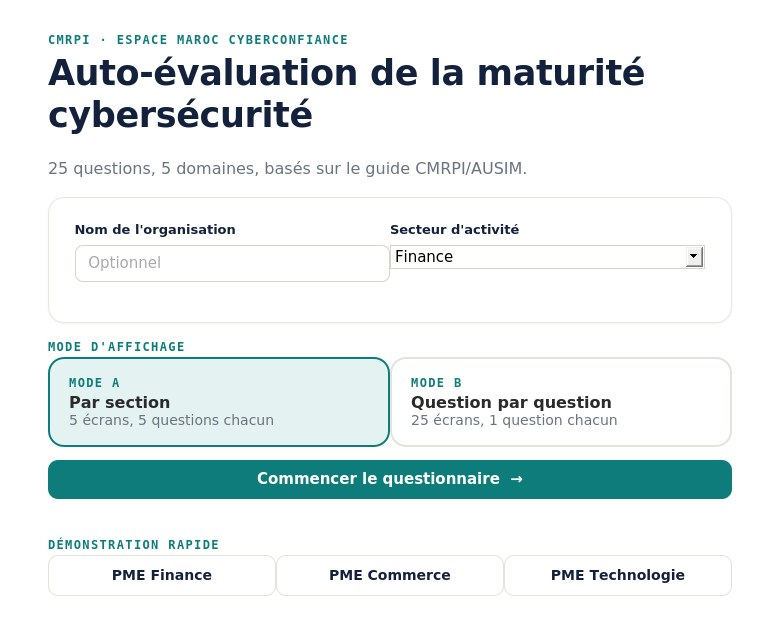
\includegraphics[width=\linewidth]{figures/01_accueil.jpg}}
    \caption{Accueil et sélection du mode}
    \label{fig:screen_home}
  \end{subfigure}
  \hfill
  \begin{subfigure}[b]{0.31\textwidth}
    \centering
    \fbox{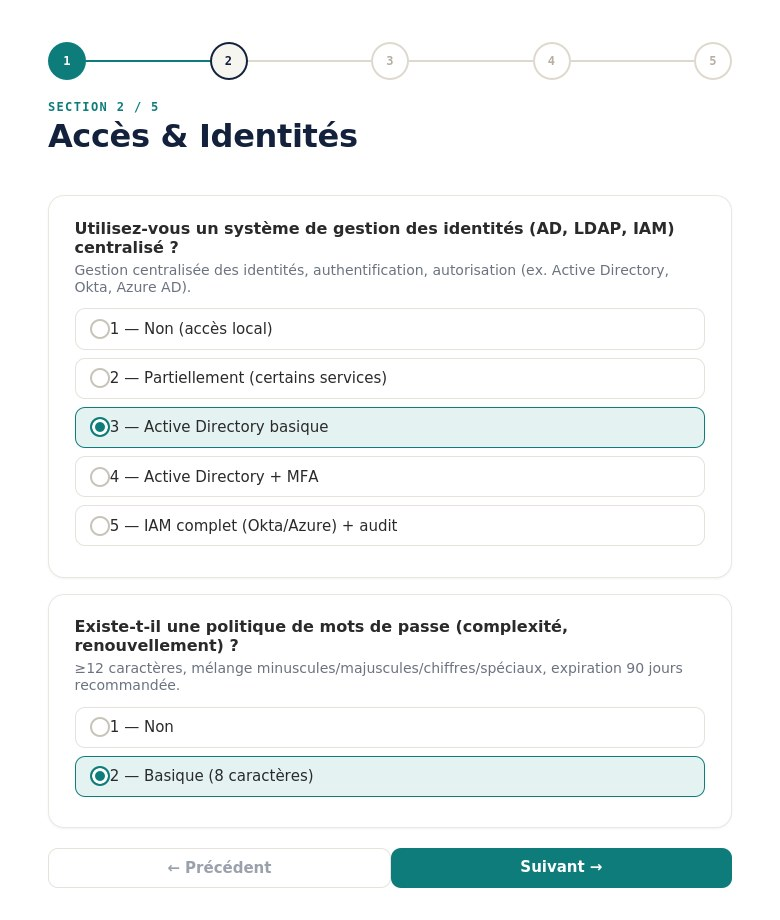
\includegraphics[width=\linewidth]{figures/02_questionnaire_section.jpg}}
    \caption{Questionnaire (mode section)}
    \label{fig:screen_questionnaire}
  \end{subfigure}
  \hfill
  \begin{subfigure}[b]{0.31\textwidth}
    \centering
    \fbox{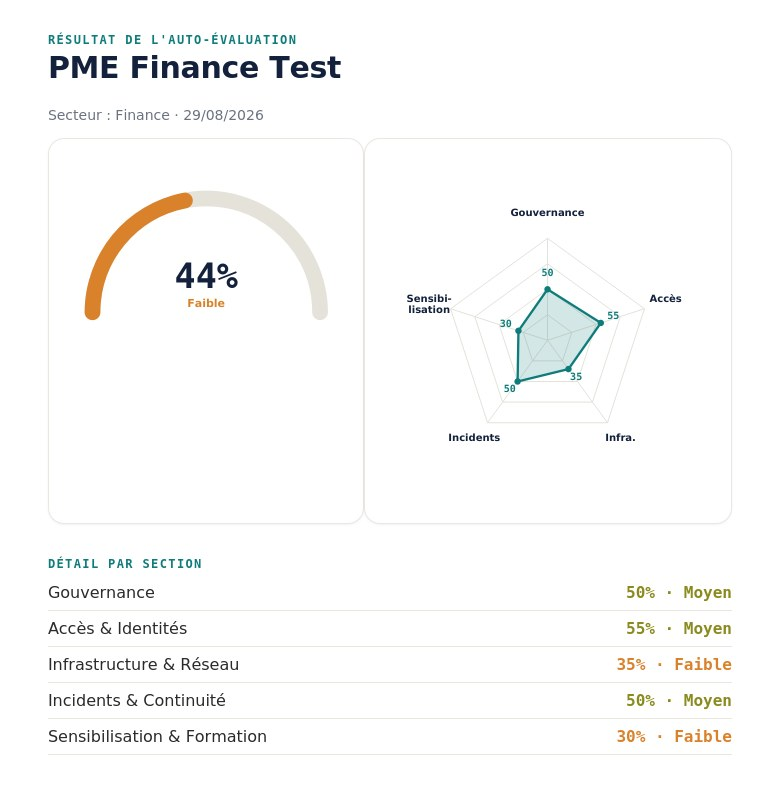
\includegraphics[width=\linewidth]{figures/03_resultats.jpg}}
    \caption{Résultats avec radar chart}
    \label{fig:screen_results}
  \end{subfigure}
  \caption{Captures d'écran des trois étapes du parcours utilisateur (profil \enquote{PME Finance Test})}
  \label{fig:screenshots}
\end{figure}

L'écran d'accueil (figure~\ref{fig:screen_home}) permet de renseigner facultativement le nom de l'organisation et son secteur, de choisir le mode d'affichage du questionnaire, et de charger instantanément un profil de démonstration. L'écran de questionnaire (figure~\ref{fig:screen_questionnaire}) illustre le mode \enquote{section}, ici pour le domaine Accès~\&~Identités : chaque question affiche son texte, un texte de guidance contextualisé et cinq options de réponse sous forme de cartes sélectionnables, avec un indicateur en pastilles matérialisant la progression à travers les cinq domaines. L'écran de résultats (figure~\ref{fig:screen_results}) affiche la jauge de score global colorée selon le niveau de maturité, le radar chart des cinq scores de domaine, ainsi que le détail par domaine. Dans les deux modes de questionnaire, le bouton \enquote{Suivant} reste désactivé tant que la section ou la question en cours n'a pas de réponse.

\subsection{Export PDF}

Le rapport de résultats généré par ReportLab (figure~\ref{fig:pdf_export}) comprend un en-tête aux couleurs du \gls{cmrpi}, un tableau d'identification de la \gls{pme}, une jauge en arc colorée selon le niveau de maturité obtenu, un graphique en barres des cinq scores de domaine, un tableau détaillé des réponses et deux à trois recommandations prioritaires accompagnées d'un badge de sévérité coloré (Critique, Haute, Moyenne, Basse).

\begin{figure}[H]
  \centering
  \begin{subfigure}[b]{0.47\textwidth}
    \centering
    \fbox{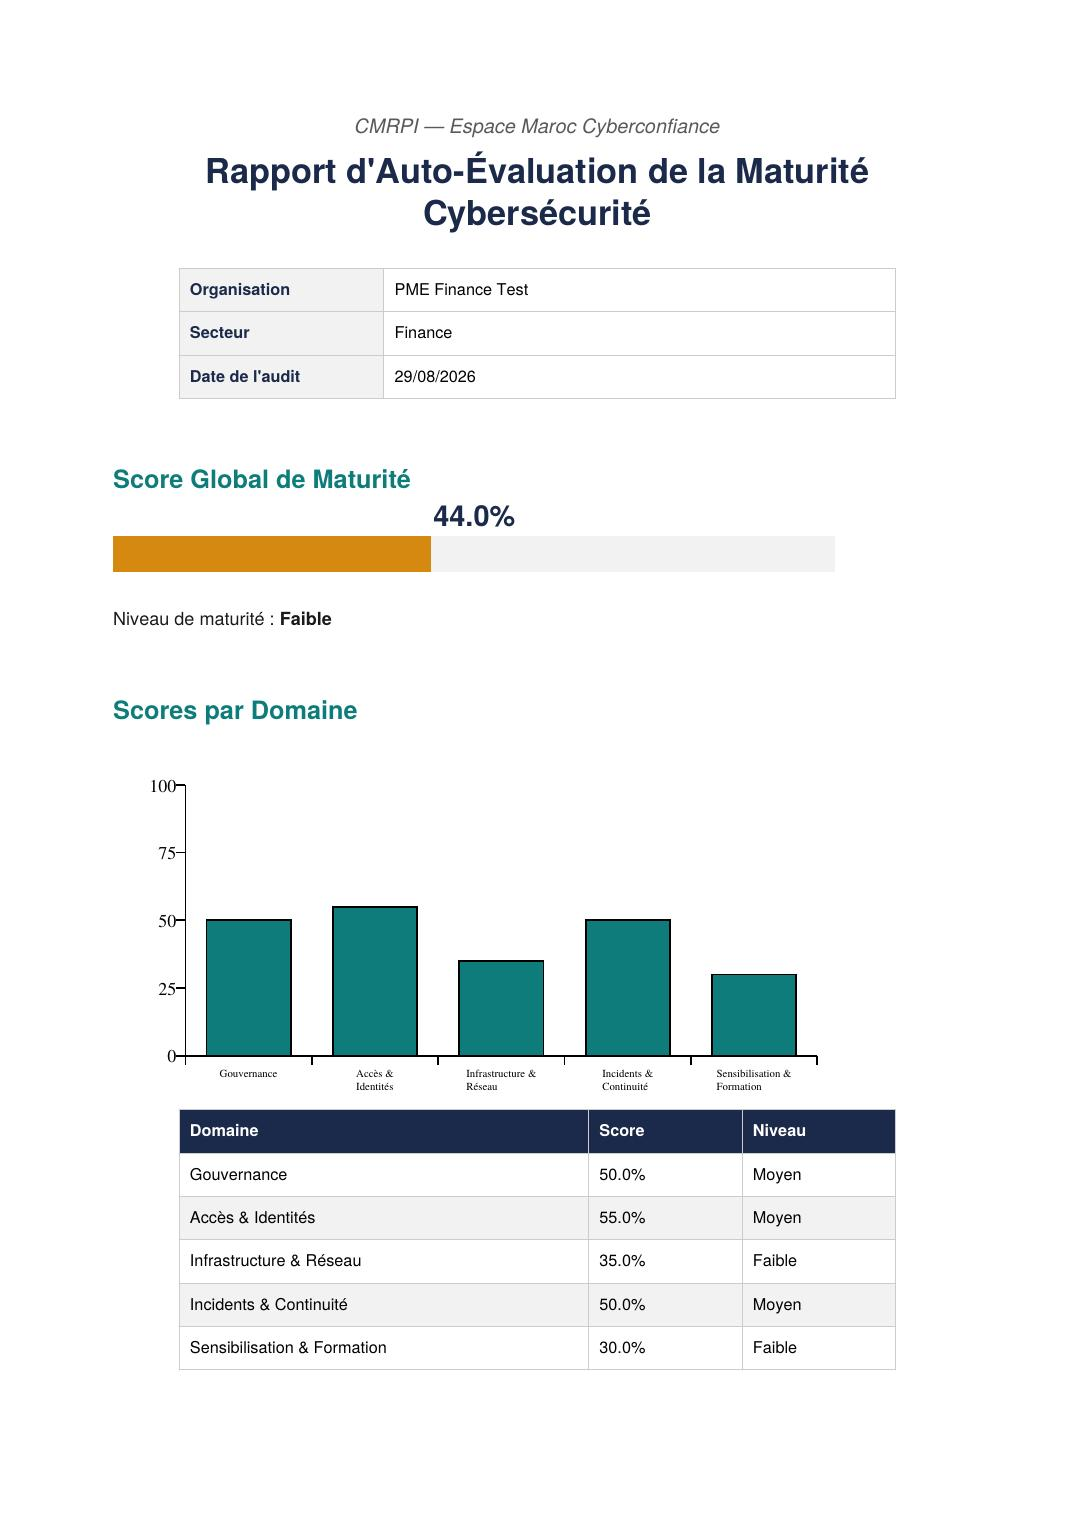
\includegraphics[width=\linewidth]{figures/pdf_page1.jpg}}
    \caption{Page 1 -- score global et scores par domaine}
    \label{fig:pdf_page1}
  \end{subfigure}
  \hfill
  \begin{subfigure}[b]{0.47\textwidth}
    \centering
    \fbox{
\includegraphics[width=\linewidth]{figures/pdf_page2.jpg}}
    \caption{Page 2 -- recommandations prioritaires}
    \label{fig:pdf_page2}
  \end{subfigure}
  \caption{Rapport PDF exporté (profil \enquote{PME Finance Test}, score global 44,0\,\%)}
  \label{fig:pdf_export}
\end{figure}

\subsection{Profils fictifs de test intégrés}

Conformément à l'exigence du brief du Jalon~2 (\enquote{tester avec 2--3 profils fictifs de \gls{pme}}), les trois profils présentés au tableau~\ref{tab:profils} peuvent être chargés en un clic depuis l'écran d'accueil, via le module \texttt{src/test\_profiles.py}, afin de faciliter les démonstrations rapides de la plateforme.

% -------------------------------------------------------
\section{Référence des modules}
\label{sec:modules}

\hspace{1cm}Cette section documente les fonctions publiques des principaux modules du dossier \texttt{src/}, à des fins de maintenabilité et de reprise du projet par un futur développeur.

\subsection{\texttt{scoring.py} -- moteur de calcul du score}

Module Python pur, sans aucune dépendance externe (ni Streamlit, ni base de données), ce qui permet de le tester et de le réutiliser indépendamment de l'interface. Le tableau~\ref{tab:mod_scoring} recense l'intégralité des neuf fonctions publiques du module, telles qu'elles figurent dans le fichier \texttt{src/scoring.py} du dépôt public à la date de rédaction de ce rapport.

\begin{longtable}{|>{\ttfamily\raggedright\scriptsize}p{4.8cm}|p{9.2cm}|}
  \caption{Fonctions publiques de \texttt{scoring.py} (dépôt public)} \label{tab:mod_scoring} \\
  \hline
  \rowcolor{iacsTableHead}
  \textcolor{white}{\textnormal{\textbf{Fonction}}} & \textcolor{white}{\textbf{Rôle}} \\
  \hline
  \endfirsthead
  \multicolumn{2}{c}{\tablename\ \thetable\ -- suite de la page précédente} \\
  \hline
  \rowcolor{iacsTableHead}
  \textcolor{white}{\textnormal{\textbf{Fonction}}} & \textcolor{white}{\textbf{Rôle}} \\
  \hline
  \endhead
  \hline
  \multicolumn{2}{r}{\textit{suite page suivante}} \\
  \endfoot
  \hline
  \endlastfoot
  calculate\_\allowbreak domain\_\allowbreak score(responses) & Calcule le score (0--100) d'un domaine à partir de ses 5 réponses Likert \\
  \hline
  \rowcolor{iacsLightGray}
  calculate\_\allowbreak domain\_\allowbreak scores(\allowbreak responses\_by\_domain) & Applique \texttt{\scriptsize calculate\_domain\_score} à chacun des domaines d'un dictionnaire \{domaine : réponses\} \\
  \hline
  calculate\_\allowbreak global\_\allowbreak score(domain\_scores) & Moyenne des scores de domaine, arrondie à une décimale \\
  \hline
  \rowcolor{iacsLightGray}
  get\_\allowbreak maturity\_\allowbreak level(score) & Retourne le niveau (Critique/Faible/Moyen/Avancé) selon le score \\
  \hline
  get\_\allowbreak severity\_\allowbreak filter(\allowbreak domain\_score) & Retourne le couple (sévérités à interroger, nombre maximal de recommandations) selon le score du domaine (seuil à 60\,\%) \\
  \hline
  \rowcolor{iacsLightGray}
  generate\_\allowbreak recommendations(\allowbreak domain\_scores,\allowbreak\ get\_recs\_fn) & Sélectionne, pour chaque domaine, les recommandations filtrées par sévérité et limitées par \texttt{\scriptsize get\_severity\_filter} -- version initiale (Jalon~2), conservée dans le module \\
  \hline
  generate\_\allowbreak top\_\allowbreak recommendations(\allowbreak domain\_scores,\allowbreak\ get\_recs\_fn,\allowbreak\ limit) & Sélectionne 2 à 3 recommandations globales priorisées, domaines les plus faibles en premier -- correctif du Jalon~3 (voir section~\ref{sec:scoring}) \\
  \hline
  score\_\allowbreak full\_\allowbreak audit(all\_responses) & Fonction principale : calcule scores de domaine, score global et niveau de maturité en un seul appel \\
  \hline
  \rowcolor{iacsLightGray}
  group\_\allowbreak responses\_\allowbreak by\_\allowbreak domain(\allowbreak responses,\allowbreak\ question\_domain\_map) & Regroupe les réponses brutes \{question\_id : valeur\} par domaine à partir de la correspondance question~$\rightarrow$~domaine \\
  \hline
\end{longtable}

\subsection{\texttt{database.py} -- accès aux données}

Toutes les fonctions de ce module utilisent un gestionnaire de contexte \texttt{get\_connection()} qui active les clés étrangères SQLite et valide automatiquement (\textit{commit}) les transactions. Le tableau~\ref{tab:mod_database} en présente les fonctions les plus significatives.

\begin{table}[H]
  \centering
  \caption{Fonctions principales de \texttt{database.py}}
  \label{tab:mod_database}
  \renewcommand{\arraystretch}{1.3}
  \small
  \begin{tabularx}{\textwidth}{|l|X|}
    \hline
    \rowcolor{iacsTableHead}
    \textcolor{white}{\textbf{Fonction}} & \textcolor{white}{\textbf{Rôle}} \\
    \hline
    \texttt{init\_database()} & Applique \texttt{data/schema.sql} (création des tables et amorçage des 5 domaines) \\
    \hline
    \rowcolor{iacsLightGray}
    \texttt{seed\_questions\_and\_domains(...)} & Charge les 25 questions depuis les fichiers JSON (idempotent) \\
    \hline
    \texttt{seed\_recommendations\_from\_xlsx(xlsx\_path)} & Charge les recommandations depuis le classeur Excel \\
    \hline
    \rowcolor{iacsLightGray}
    \texttt{create\_audit(pme\_id)} / \texttt{complete\_audit(...)} & Création d'un audit et clôture avec son score final \\
    \hline
    \texttt{save\_response(...)} & Enregistre une réponse individuelle à une question \\
    \hline
    \rowcolor{iacsLightGray}
    \texttt{get\_audit\_history(pme\_id)} & Historique des audits réalisés par une \gls{pme} \\
    \hline
    \texttt{log\_action(pme\_id, action, details)} & Journalisation d'une action dans \texttt{audit\_log} \\
    \hline
  \end{tabularx}
\end{table}

\subsection{Autres modules}

Le module \texttt{auth.py} fournit le hachage et la vérification bcrypt des mots de passe, ainsi que l'inscription et l'authentification d'une \gls{pme} ; il est fonctionnel et testé, mais n'est pas branché au flux principal de l'application, l'accès direct au questionnaire sans connexion ayant été retenu pour une expérience \enquote{simple à utiliser} conforme au brief du Jalon~2. Le module \texttt{questionnaire.py} charge les 25 questions et leur guidance depuis les fichiers JSON, et expose les regroupements par domaine utilisés par le mode \enquote{section}. Le module \texttt{pdf\_generator.py} construit le rapport \gls{pdf} via sa fonction principale \texttt{generate\_\allowbreak audit\_\allowbreak report(...)}, qui reçoit désormais une liste plate de recommandations plutôt qu'un dictionnaire par domaine, conformément à \texttt{scoring.\allowbreak generate\_\allowbreak top\_\allowbreak recommendations()}. Le module \texttt{ui\_components.py} centralise le système de design (feuille de style CSS, sélecteur de mode, indicateur de progression, génération du radar chart et de la jauge en \gls{svg}). Enfin, \texttt{test\_profiles.py} définit les trois profils fictifs de démonstration et leur conversion en réponses individuelles.

% -------------------------------------------------------
\section{Tests et validation}
\label{sec:tests}

\hspace{1cm}La qualité logicielle de la plateforme a été validée par une suite de 52 tests automatisés, atteignant 90\,\% de couverture de code (mesurée avec pytest-cov). Ces tests couvrent le moteur de scoring, l'authentification, la base de données, la génération \gls{pdf} et le questionnaire. Le tableau~\ref{tab:tests} détaille leur répartition par fichier.

\begin{table}[H]
  \centering
  \caption{Répartition de la suite de tests}
  \label{tab:tests}
  \renewcommand{\arraystretch}{1.3}
  \small
  \begin{tabularx}{\textwidth}{|l|c|X|}
    \hline
    \rowcolor{iacsTableHead}
    \textcolor{white}{\textbf{Fichier}} &
    \textcolor{white}{\textbf{Tests}} &
    \textcolor{white}{\textbf{Contenu}} \\
    \hline
    \texttt{test\_scoring.py} & 15 & Formules de score, seuils de maturité, sélection de recommandations \\
    \hline
    \rowcolor{iacsLightGray}
    \texttt{test\_questionnaire.py} & 8 & Chargement JSON, validation des réponses \\
    \hline
    \texttt{test\_profiles.py} & 3 & Cohérence des 3 profils de démonstration \\
    \hline
    \rowcolor{iacsLightGray}
    \texttt{test\_auth.py} & 8 & Inscription, connexion, hachage des mots de passe \\
    \hline
    \texttt{test\_database\_pdf.py} & 6 & CRUD base de données, génération \gls{pdf} \\
    \hline
    \rowcolor{iacsLightGray}
    \texttt{test\_app\_flow.py} & 12 & Tests de bout en bout (\texttt{AppTest}) : parcours complet, 2 modes, export \gls{pdf} \\
    \hline
    \textbf{Total} & \textbf{52} & \\
    \hline
  \end{tabularx}
\end{table}

Les tests de bout en bout utilisent \texttt{streamlit.testing.v1.AppTest}, le framework officiel Streamlit qui simule un utilisateur réel cliquant dans l'application, sans navigateur ni serveur à lancer manuellement. Ils couvrent notamment le chargement de l'accueil sans erreur, les trois profils de démonstration affichant le score exact attendu, la désactivation du bouton \enquote{Suivant} tant qu'une réponse manque, le parcours complet dans les deux modes jusqu'à l'écran de score, et la présence du bouton de téléchargement \gls{pdf} en fin de parcours.

Le code respecte par ailleurs les règles de style PEP~8, avec zéro erreur relevée par flake8 (longueur de ligne maximale fixée à 120 caractères dans \texttt{setup.cfg}). Un pipeline d'intégration continue (\texttt{.github/workflows/ci.yml}) exécute automatiquement, à chaque \textit{push} ou \textit{pull request}, l'installation des dépendances, la vérification flake8 sur \texttt{src/}, \texttt{app.py} et \texttt{tests/}, ainsi que l'ensemble de la suite pytest avec couverture, sur un environnement Python~3.12 entièrement vierge.

\iacswarning{Une vérification d'installation sur environnement vierge a révélé, au Jalon~3, trois régressions de dépendances : la bibliothèque \texttt{pandas}, non utilisée dans le code mais cassant l'installation sur Python~3.12 ; une version de \texttt{streamlit} trop ancienne, cassant les tests \texttt{AppTest} ; et une version de \texttt{flake8} trop ancienne générant de faux positifs sur les f-strings. Ces trois régressions ont été corrigées, revérifiées de bout en bout, et sont désormais prévenues par le pipeline d'intégration continue.}

% -------------------------------------------------------
\section{Fonctionnalités au-delà du périmètre strict}
\label{sec:bonus}

Deux fonctionnalités ont été développées au-delà du périmètre strict initialement défini : un module d'authentification par hachage bcrypt avec persistance multi-audits (historique des évaluations d'une même \gls{pme}), et l'export \gls{pdf}, qui est devenu périmètre officiel dès le Jalon~3. Ces éléments illustrent une anticipation des besoins au-delà du cahier des charges initial ; il convient toutefois de préciser que le module d'authentification n'est, à ce stade, pas pleinement intégré au flux principal validé.

% -------------------------------------------------------
\section{Résultats obtenus}
\label{sec:resultats}

Au terme du stage, la plateforme constitue un système fonctionnel de bout en bout, couvrant le parcours complet questionnaire~$\rightarrow$~score~$\rightarrow$~export \gls{pdf}. Elle a été validée par l'encadrant professionnel à chaque jalon, avec des retours explicites (\enquote{bravo, un livrable de qualité} au Jalon~1, \enquote{merci pour les résultats} au Jalon~2). Le code source est public et documenté à l'adresse \url{https://github.com/YOUSSEFKARROUM/PFA_CRMPI}, accompagné d'une documentation technique dédiée couvrant l'architecture, le guide d'installation, la référence des modules et le dépannage. Sur le plan de la qualité logicielle, le projet compte 52 tests automatisés, 90\,\% de couverture de code, un pipeline \gls{ci} opérationnel et une dette technique de lint nulle.

% -------------------------------------------------------
\section{Limites observées}
\label{sec:limites}

Plusieurs limites ont été identifiées à l'issue du stage :

\begin{itemize}
  \item Le périmètre reste mono-utilisateur ; le support multi-tenant complet n'est pas implémenté en production.
  \item La base SQLite n'est pas adaptée à une montée en charge au-delà d'une cinquantaine d'utilisateurs concurrents ; une migration vers PostgreSQL est identifiée comme nécessaire pour un passage en production.
  \item Le benchmarking anonymisé inter-\gls{pme} n'est pas encore implémenté.
  \item La plateforme n'est aujourd'hui exécutée qu'en local ; le déploiement en ligne reste à réaliser (voir ci-dessous).
\end{itemize}

% -------------------------------------------------------
\section{Perspectives d'amélioration}
\label{sec:perspectives}

Plusieurs pistes d'évolution ont été identifiées, certaines en concertation avec l'encadrant.

\textbf{Déploiement en ligne.} La procédure prévue -- non encore réalisée au moment de la rédaction de ce rapport -- consiste à déployer la plateforme sur Streamlit Community Cloud, l'option la plus rapide pour donner un accès en ligne à l'encadrant : création d'une application depuis le dépôt GitHub public (branche \texttt{main}, fichier \texttt{app.py}), installation automatique de \texttt{requirements.txt}, et initialisation automatique de la base au premier lancement si \texttt{app.db} n'existe pas encore. Un point de vigilance a toutefois été identifié : le système de fichiers de Streamlit Community Cloud n'est pas garanti persistant entre redéploiements, ce qui rend la migration vers une base hébergée (par exemple PostgreSQL managé) nécessaire au-delà d'un usage de démonstration.

\begin{enumerate}
  \item Migrer de Streamlit vers une architecture Django ou FastAPI côté serveur avec un frontend React, pour une version production multi-utilisateurs.
  \item Migrer la base de données de SQLite vers PostgreSQL, notamment pour garantir la persistance des données en déploiement cloud.
  \item Finaliser le déploiement sur Streamlit Community Cloud selon la procédure décrite ci-dessus.
  \item Mettre en place un benchmarking sectoriel anonymisé entre \gls{pme}.
  \item Étudier la faisabilité d'une certification \enquote{PME Cyber-Sûre}, piste évoquée avec l'encadrant.
  \item Étendre le questionnaire à des \textit{tracks} sectoriels spécialisés (Finance, Santé, E-commerce).
\end{enumerate}

\section*{Conclusion}

Ce chapitre a présenté la conception et la réalisation de la plateforme d'auto-évaluation de la maturité cybersécurité : architecture technique, modélisation des données et du questionnaire, méthodologie de scoring justifiée académiquement, réalisation de l'interface et de l'export \gls{pdf}, ainsi que les tests et résultats obtenus. Les limites observées et les perspectives identifiées tracent les prochaines étapes envisageables pour faire évoluer cette plateforme vers un usage en production.


% --- Conclusion générale ---
% ============================================================
%  CONCLUSION GÉNÉRALE
% ============================================================
\chapter*{Conclusion générale et perspectives}
\addcontentsline{toc}{chapter}{Conclusion générale et perspectives}
\markboth{Conclusion générale}{Conclusion générale}

\hspace{1cm}Ce stage de Projet de Fin d'Année, réalisé sur sept semaines (15~juillet -- 31~août~2026) au sein du \gls{cmrpi} -- Espace Maroc Cyberconfiance, a porté sur la conception et le développement d'une plateforme d'auto-évaluation de la maturité cybersécurité destinée aux \gls{pme} marocaines. Au terme de ce travail, je peux dresser le bilan suivant.

\vspace{0.5cm}
\textbf{Bilan des réalisations :}

\begin{itemize}
  \item Une analyse des référentiels normatifs (guide \gls{cmrpi}/\gls{ausim}, \gls{iso27001}, \gls{nistcsf}, loi 09-08) a permis de justifier académiquement une structure de questionnaire en 5 domaines et 25 questions.
  \item Une plateforme fonctionnelle a été conçue et développée, intégrant un questionnaire d'auto-évaluation, un moteur de scoring automatisé et reproductible, ainsi qu'un export de rapports personnalisés au format \gls{pdf}.
  \item La qualité logicielle de la plateforme a été validée par 52 tests automatisés, 90\,\% de couverture de code et un pipeline d'intégration continue, avec une validation de la cohérence méthodologique sur trois profils fictifs de \gls{pme}.
  \item La démarche a été menée en trois jalons itératifs, avec un suivi hebdomadaire et une validation systématique par l'encadrant professionnel, le Dr.~Rachid Abouettahir.
\end{itemize}

\vspace{0.5cm}
\textbf{Compétences mobilisées :} analyse de référentiels normatifs en cybersécurité, conception d'une méthodologie de scoring justifiée académiquement, développement full-stack en Python, mise en place de tests automatisés et d'un pipeline d'intégration continue, gestion de projet et communication avec un encadrant professionnel.

\vspace{0.5cm}
\textbf{Perspectives :}

\begin{enumerate}
  \item Migrer l'architecture vers Django ou FastAPI côté serveur avec un frontend React, pour une version production multi-utilisateurs.
  \item Migrer la base de données de SQLite vers PostgreSQL afin de supporter une montée en charge.
  \item Déployer la plateforme sur Streamlit Community Cloud et finaliser la documentation technique.
  \item Mettre en place un benchmarking sectoriel anonymisé entre \gls{pme} et étudier la faisabilité d'une certification \enquote{PME Cyber-Sûre}.
\end{enumerate}

\vspace{0.5cm}
Au-delà du livrable technique, ce stage illustre l'impact potentiel d'une telle plateforme pour sensibiliser les \gls{pme} marocaines à leur maturité cybersécurité, en cohérence directe avec la mission du \gls{cmrpi}.



% %%%%%%%%%%%%%%%%%%%%%%%%%%%%%%%%%%%%%%%%%%%%%%%%%%%%%%%%%%%%
%  BIBLIOGRAPHIE
% %%%%%%%%%%%%%%%%%%%%%%%%%%%%%%%%%%%%%%%%%%%%%%%%%%%%%%%%%%%%
\printbibliography[heading=bibintoc, title={Bibliographie}]


% %%%%%%%%%%%%%%%%%%%%%%%%%%%%%%%%%%%%%%%%%%%%%%%%%%%%%%%%%%%%
%  ANNEXES
% %%%%%%%%%%%%%%%%%%%%%%%%%%%%%%%%%%%%%%%%%%%%%%%%%%%%%%%%%%%%
\appendix

\chapter*{Annexes}
\addcontentsline{toc}{chapter}{Annexes}
\markboth{Annexes}{Annexes}

\section*{Annexe A : Guide d'installation}

\subsection*{A.1 Prérequis}

\begin{itemize}
  \item Python 3.12 ou supérieur ;
  \item Node.js 22 ou supérieur (pour compiler l'interface) ;
  \item pip (gestionnaire de paquets Python) ;
  \item git.
\end{itemize}

\subsection*{A.2 Étapes d'installation}

\begin{lstlisting}[language=bash, caption={Installation et lancement de la plateforme}, basicstyle=\ttfamily\footnotesize\color{iacsDark}, frame=l]
# 1. Cloner le repository
git clone https://github.com/YOUSSEFKARROUM/PFA_CRMPI.git cmrpi-platform
cd cmrpi-platform

# 2. Creer un environnement virtuel (recommande)
python3 -m venv venv
source venv/bin/activate      # Windows : venv\Scripts\activate

# 3. Installer les dependances
pip install -r requirements.txt
pip install -r requirements-dev.txt   # pour les tests et le lint

# 4. Compiler l'interface React
cd frontend && npm ci && npm run build && cd ..

# 5. Lancer l'application (la base app.db est creee au demarrage)
uvicorn api.main:app --port 8000
# -> disponible sur http://localhost:8000

# 6. Verifier l'installation (optionnel)
pytest --cov=src --cov=api          # -> "285 passed" attendu
cd frontend && npm run test:coverage && npm run test:e2e
\end{lstlisting}

Au démarrage, l'application crée et alimente automatiquement la base ; le script \texttt{scripts/init\_db.py} permet de le faire à la main. Il crée le fichier \texttt{app.db} à partir de \texttt{data/schema.sql}, puis charge les 25 questions (français/anglais et guidance) ainsi que les recommandations depuis le classeur Excel \texttt{data/recommendations/Recommendations\_Database.xlsx}.

\section*{Annexe B : Schéma de la base de données}

Le tableau~\ref{tab:annexe_schema} détaille les colonnes des deux tables centrales du modèle, \texttt{pme} et \texttt{audit} ; le schéma complet des sept tables (\texttt{pme}, \texttt{domain}, \texttt{question}, \texttt{audit}, \texttt{audit\_response}, \texttt{recommendation}, \texttt{audit\_log}) est disponible dans \texttt{data/schema.sql} du dépôt.

\renewcommand{\thetable}{B.1}
\begin{table}[H]
  \centering
  \caption{Colonnes de la table \texttt{pme}}
  \label{tab:annexe_schema}
  \renewcommand{\arraystretch}{1.3}
  \small
  \begin{tabularx}{\textwidth}{|l|l|X|}
    \hline
    \rowcolor{iacsTableHead}
    \textcolor{white}{\textbf{Colonne}} &
    \textcolor{white}{\textbf{Type}} &
    \textcolor{white}{\textbf{Description}} \\
    \hline
    \texttt{id} & TEXT (UUID) PK & Identifiant unique \\
    \hline
    \rowcolor{iacsLightGray}
    \texttt{email} & TEXT UNIQUE & Email de connexion \\
    \hline
    \texttt{password\_hash} & TEXT & Mot de passe haché (bcrypt) \\
    \hline
    \rowcolor{iacsLightGray}
    \texttt{name}, \texttt{sector} & TEXT & Nom de l'organisation, secteur d'activité \\
    \hline
    \texttt{created\_at} & DATETIME & Horodatage de création \\
    \hline
  \end{tabularx}
\end{table}

\renewcommand{\thetable}{B.2}
\begin{table}[H]
  \centering
  \caption{Colonnes de la table \texttt{audit}}
  \renewcommand{\arraystretch}{1.3}
  \small
  \begin{tabularx}{\textwidth}{|l|l|X|}
    \hline
    \rowcolor{iacsTableHead}
    \textcolor{white}{\textbf{Colonne}} &
    \textcolor{white}{\textbf{Type}} &
    \textcolor{white}{\textbf{Description}} \\
    \hline
    \texttt{id} & TEXT (UUID) PK & Identifiant de l'audit \\
    \hline
    \rowcolor{iacsLightGray}
    \texttt{pme\_id} & TEXT FK & \gls{pme} concernée \\
    \hline
    \texttt{global\_score} & REAL & Score global calculé (0--100) \\
    \hline
    \rowcolor{iacsLightGray}
    \texttt{completed\_at} & DATETIME & Date de complétion (NULL si en cours) \\
    \hline
  \end{tabularx}
\end{table}

\section*{Annexe C : Extrait du questionnaire (format JSON)}

Les questions, leur texte d'aide et leurs traductions sont pilotées par les fichiers JSON du dossier \texttt{data/questions/}. L'extrait ci-dessous illustre le format retenu pour une question du domaine Gouvernance.

\begin{lstlisting}[language=Python, caption={Extrait de \texttt{questions\_fr.json}}, basicstyle=\ttfamily\footnotesize\color{iacsDark}, frame=l]
{
  "id": "q_gov_01",
  "domain_id": "dom_gov",
  "order": 1,
  "text": "Votre organisation dispose-t-elle d'une politique de securite formalisee ?",
  "options": [
    {"value": 1, "label": "Non"},
    {"value": 2, "label": "Partiellement"},
    {"value": 3, "label": "Approuvee (1-2 ans)"},
    {"value": 4, "label": "Approuvee + revue annuelle"},
    {"value": 5, "label": "Approuvee + revue + communiquee"}
  ]
}
\end{lstlisting}

\section*{Annexe D : Dépannage (extrait de la documentation technique)}

Le tableau~\ref{tab:annexe_faq} reprend les principaux incidents rencontrés au cours du développement, documentés à des fins de maintenabilité pour un futur développeur reprenant le projet.

\renewcommand{\thetable}{D.1}
\begin{table}[H]
  \centering
  \caption{Foire aux questions -- incidents rencontrés et solutions}
  \label{tab:annexe_faq}
  \renewcommand{\arraystretch}{1.4}
  \small
  \begin{tabularx}{\textwidth}{|X|X|}
    \hline
    \rowcolor{iacsTableHead}
    \textcolor{white}{\textbf{Symptôme}} &
    \textcolor{white}{\textbf{Cause et solution}} \\
    \hline
    \texttt{pip install} échoue avec une erreur \texttt{pkg\_resources} sous Python 3.12 & Une ancienne version de \texttt{pandas} (2.0.3), pourtant inutilisée dans le code, était épinglée dans \texttt{requirements.txt} et ne s'installait pas sur Python 3.12. Retirée du fichier. \\
    \hline
    \rowcolor{iacsLightGray}
    Le score affiché ne change pas après modification du navigateur & Comportement voulu : le serveur ignore tout score envoyé par le client et recalcule toujours à partir des réponses brutes. \\
    \hline
    Prototype Streamlit : flake8 remontait des centaines de fausses erreurs sur \texttt{ui\_components.py} & flake8~6.0.0 associé à pycodestyle~2.10 interprète mal le contenu CSS à l'intérieur des f-strings sur Python~3.12 (changement de tokenisation PEP~701). Le projet est contraint sur \texttt{flake8>=7.0}. \\
    \hline
    \rowcolor{iacsLightGray}
    \texttt{app.db} corrompue ou incohérente & Supprimer le fichier et relancer l'initialisation : \texttt{rm app.db \&\& python scripts/init\_db.py}. \\
    \hline
    Le PDF généré affiche des caractères accentués incorrects & Vérifier l'encodage UTF-8 du classeur \texttt{Recommendations\_Database.xlsx} ; incident similaire déjà rencontré et corrigé au Jalon~2. \\
    \hline
  \end{tabularx}
\end{table}

\end{document}
